%%%%%%%%%%%%%%%%%%%%%%%%%%%%%%%%%%%%%%%%%%%%%%%%%%%%%%%%%%%%%%%%%%%%%%%%%%%%%%%%
%% Plantilla de memoria en LaTeX para la EIF - Universidad Rey Juan Carlos
%%
%% Por Gregorio Robles <grex arroba gsyc.urjc.es>
%%     Grupo de Sistemas y Comunicaciones
%%     Escuela de Ingeniería de Fuenlabrada
%%     Universidad Rey Juan Carlos
%% (muchas ideas tomadas de Internet, colegas del GSyC, antiguos alumnos...
%%  etc. Muchas gracias a todos)
%%
%% La última versión de esta plantilla está siempre disponible en:
%%     https://github.com/gregoriorobles/plantilla-memoria
%%
%% Para obtener PDF, ejecuta en la shell:
%%   make
%% (las imágenes deben ir en PNG o JPG)

%%%%%%%%%%%%%%%%%%%%%%%%%%%%%%%%%%%%%%%%%%%%%%%%%%%%%%%%%%%%%%%%%%%%%%%%%%%%%%%%

\documentclass[a4paper, 12pt]{book}
%\usepackage[T1]{fontenc}

\usepackage{textcomp}
\usepackage[hidelinks]{hyperref}
\usepackage{xcolor}
\usepackage[a4paper, left=2.5cm, right=2.5cm, top=3cm, bottom=3cm]{geometry}
\usepackage{times}
\usepackage[utf8]{inputenc}
\usepackage[spanish]{babel} % Comenta esta línea si tu memoria es en inglés
\usepackage{url}
\usepackage{listings}
%\usepackage[dvipdfm]{graphicx}
\usepackage{graphicx}
\usepackage{caption}
\usepackage{float}  %% H para posicionar figuras
\usepackage[nottoc, notlot, notlof, notindex]{tocbibind} %% Opciones de índice
\usepackage{latexsym}  %% Logo LaTeX

\definecolor{codegray}{RGB}{100,100,100} % Puedes ajustar el gris aquí

\lstset{
  basicstyle=\ttfamily\scriptsize\color{codegray},
  showstringspaces=false,
  breaklines=true,
  numbers=none,
  language={},        
  keywordstyle=,
  commentstyle=,
  stringstyle=,
  identifierstyle=,
}

% Escribe el título y el nombre del autor / autora para que se use bien
% en otras partes de la plantilla
% Dependiendo de las partes de la plantilla, a veces aparecerán tal
% cual los escribas, a veces totalmente en mayúsculas, a veces de otras
% formas
\title{Título del Trabajo con Letras Mayúsculas para Sustantivos y Adjetivos}
\author{Juan José Arias Rojas}

% Guarda el título, el autor y la fecha en variables
\makeatletter
\let\thetitle\@title
\let\theauthor\@author
\let\thedate\@date
\makeatother

\renewcommand{\baselinestretch}{1.5}  %% Interlineado

\begin{document}

\renewcommand{\refname}{Bibliografía}  %% Renombrando
\renewcommand{\appendixname}{Apéndice}


%%%%%%%%%%%%%%%%%%%%%%%%%%%%%%%%%%%%%%%%%%%%%%%%%%%%%%%%%%%%%%%%%%%%%%%%%%%%%%%%
% PORTADA

\begin{titlepage}
	\begin{center}
		\includegraphics[scale=0.6]{img/URJ_logo_Color_POS.png}

		\vspace{1.75cm}

		\LARGE
		ESCUELA DE INGENIERÍA DE FUENLABRADA
		\vspace{1cm}

		\LARGE
		GRADO EN INGENÍERIA EN SISTEMAS AUDIOVISUALES Y MULTIMEDIA

		\vspace{1cm}
		\LARGE
		\textbf{TRABAJO FIN DE GRADO}

		\vspace{2cm}

		\Large
		\MakeUppercase{\thetitle}

		\vspace{2cm}

		\large
		Autor : \theauthor \\
		Tutor : Dr. Jesús María González Barahona\\
		\vspace{1cm}

		\large
		Curso académico 2024/2025

	\end{center}
\end{titlepage}

\newpage
\mbox{}
\thispagestyle{empty} % para que no se numere esta pagina



%%%%%%%%%%%%%%%%%%%%%%%%%%%%%%%%%%%%%%%%%%%%%%%%%%%%%%%%%%%%%%%%%%%%%%%%%%%%%%%%
%%%% Licencia
\clearpage
\pagenumbering{gobble}
\chapter*{}

\vspace{12cm}


\begin{flushright}
	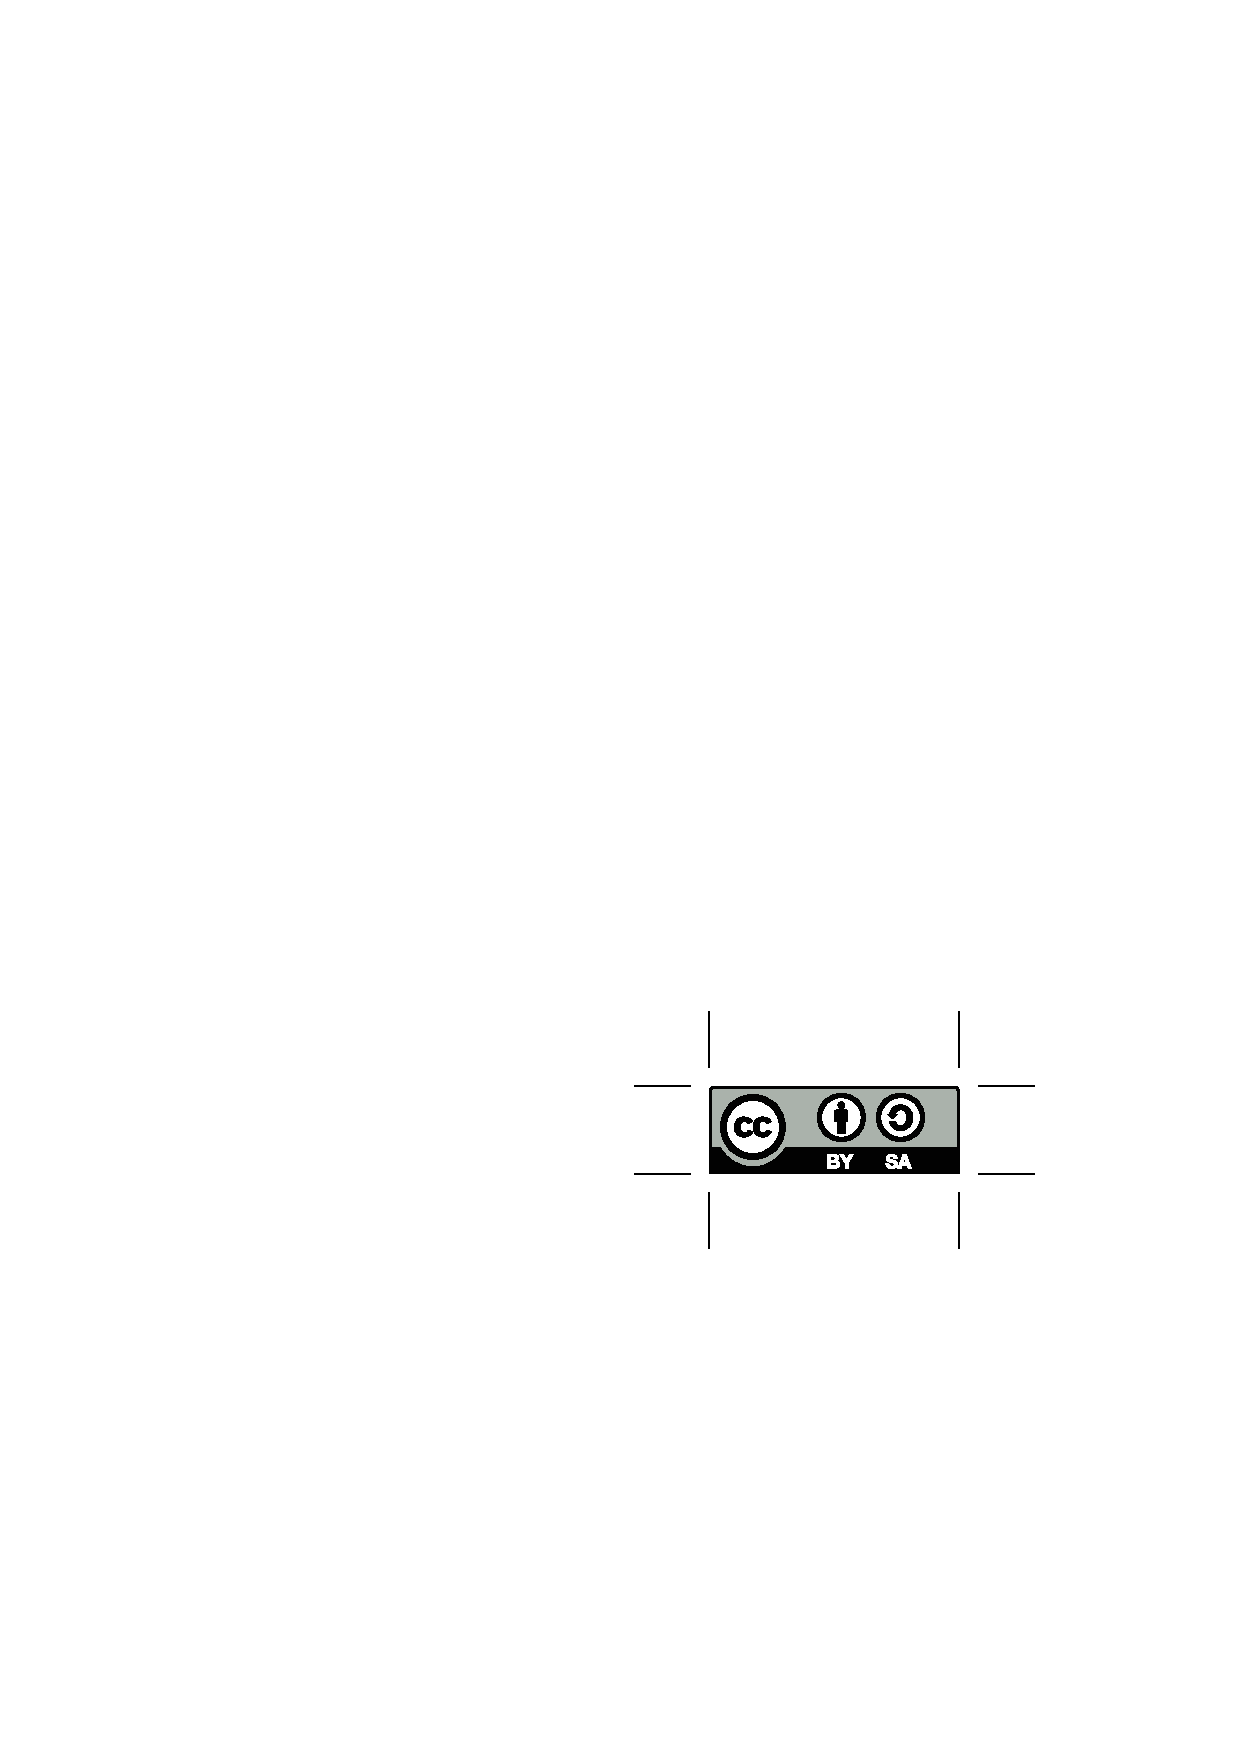
\includegraphics[scale=0.6]{img/by-sa}
	%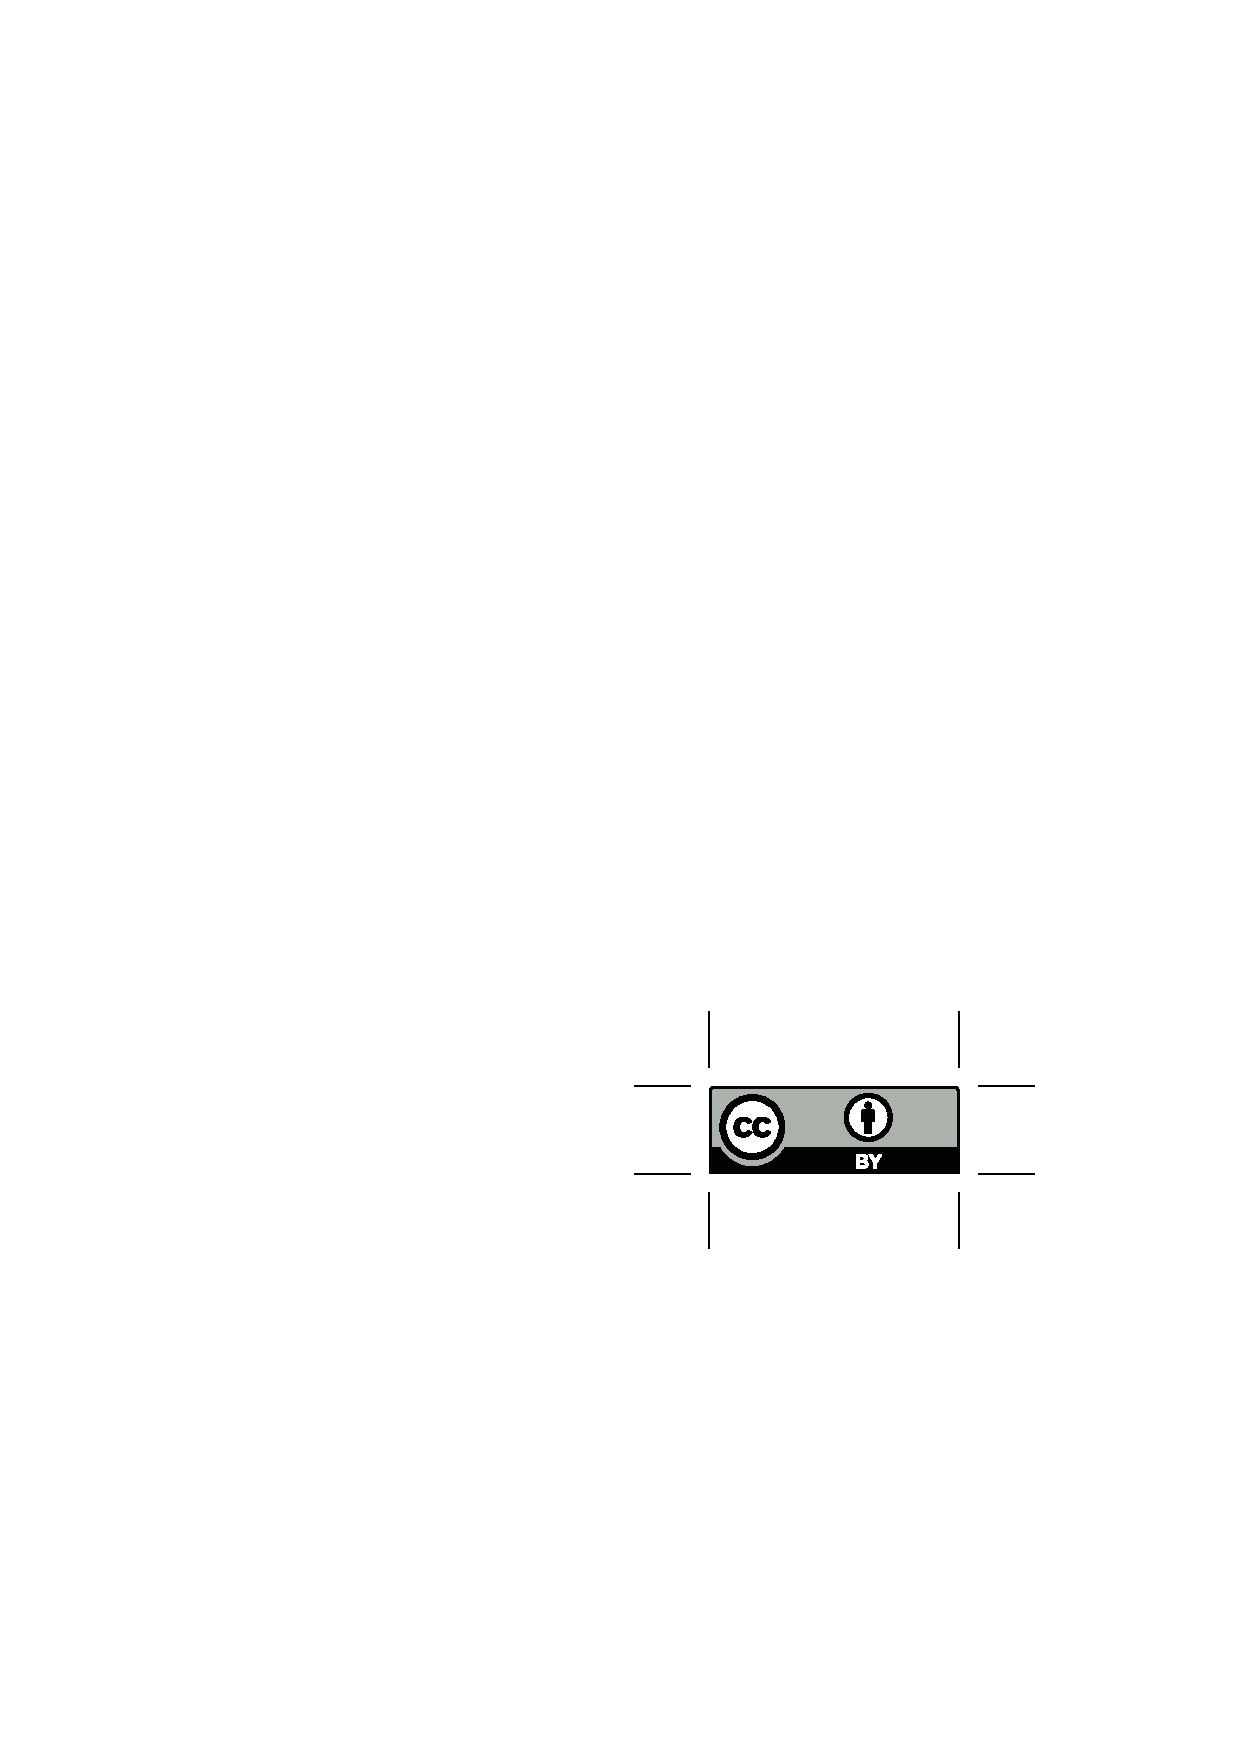
\includegraphics[scale=0.6]{img/by}

	%% Poner el año adecuado
	\noindent©2025 \theauthor  \\
	Algunos derechos reservados  \\
	Este documento se distribuye bajo la licencia \\
	``Atribución-CompartirIgual 4.0 Internacional'' de Creative Commons, \\
	disponible en \\
	\url{https://creativecommons.org/licenses/by-sa/4.0/deed.es}
\end{flushright}

%%%%%%%%%%%%%%%%%%%%%%%%%%%%%%%%%%%%%%%%%%%%%%%%%%%%%%%%%%%%%%%%%%%%%%%%%%%%%%%%
%%%% Dedicatoria

\chapter*{}
\pagenumbering{Roman} % para comenzar la numeracion de paginas en numeros romanos
\begin{flushright}
	\textit{Dedicado a \\
		todos aquellos que me animaron y apollaron \\
		incluso en mis momentos de debilidad}
\end{flushright}

%%%%%%%%%%%%%%%%%%%%%%%%%%%%%%%%%%%%%%%%%%%%%%%%%%%%%%%%%%%%%%%%%%%%%%%%%%%%%%%%
%%%% Agradecimientos

\chapter*{Agradecimientos}
%\addcontentsline{toc}{chapter}{Agradecimientos} % si queremos que aparezca en el índice
\markboth{AGRADECIMIENTOS}{AGRADECIMIENTOS} % encabezado 


%%%%%%%%%%%%%%%%%%%%%%%%%%%%%%%%%%%%%%%%%%%%%%%%%%%%%%%%%%%%%%%%%%%%%%%%%%%%%%%%
%%%% Resumen

\chapter*{Resumen}
%\addcontentsline{toc}{chapter}{Resumen} % si queremos que aparezca en el índice
\markboth{RESUMEN}{RESUMEN} % encabezado


%%%%%%%%%%%%%%%%%%%%%%%%%%%%%%%%%%%%%%%%%%%%%%%%%%%%%%%%%%%%%%%%%%%%%%%%%%%%%%%%
%%%% Resumen en inglés

\chapter*{Summary}
%\addcontentsline{toc}{chapter}{Summary} % si queremos que aparezca en el índice
\markboth{SUMMARY}{SUMMARY} % encabezado

%%%%%%%%%%%%%%%%%%%%%%%%%%%%%%%%%%%%%%%%%%%%%%%%%%%%%%%%%%%%%%%%%%%%%%%%%%%%%%%%
%%%%%%%%%%%%%%%%%%%%%%%%%%%%%%%%%%%%%%%%%%%%%%%%%%%%%%%%%%%%%%%%%%%%%%%%%%%%%%%%
% ÍNDICES %
%%%%%%%%%%%%%%%%%%%%%%%%%%%%%%%%%%%%%%%%%%%%%%%%%%%%%%%%%%%%%%%%%%%%%%%%%%%%%%%%

% Las buenas noticias es que los índices se generan automáticamente.
% Lo único que tienes que hacer es elegir cuáles quieren que se generen,
% y comentar/descomentar esa instrucción de LaTeX.

%%%% Índice de contenidos
\tableofcontents
%%%% Índice de figuras
\cleardoublepage
%\addcontentsline{toc}{chapter}{Lista de figuras} % para que aparezca en el indice de contenidos
\listoffigures % indice de figuras
%%%% Índice de tablas
%\cleardoublepage
%\addcontentsline{toc}{chapter}{Lista de tablas} % para que aparezca en el indice de contenidos
%\listoftables % indice de tablas


%%%%%%%%%%%%%%%%%%%%%%%%%%%%%%%%%%%%%%%%%%%%%%%%%%%%%%%%%%%%%%%%%%%%%%%%%%%%%%%%
%%%%%%%%%%%%%%%%%%%%%%%%%%%%%%%%%%%%%%%%%%%%%%%%%%%%%%%%%%%%%%%%%%%%%%%%%%%%%%%%
% INTRODUCCIÓN cpitulo 1%
%%%%%%%%%%%%%%%%%%%%%%%%%%%%%%%%%%%%%%%%%%%%%%%%%%%%%%%%%%%%%%%%%%%%%%%%%%%%%%%%

\cleardoublepage
\chapter{Introducción}
\label{sec:intro} % etiqueta para poder referenciar luego en el texto con ~\ref{sec:intro}
\pagenumbering{arabic} % para empezar la numeración de página con números
La realidad virtual es un campo que cada vez toma mayor peso, e introducir al usuario cada vez más dentro del entorno virtual ha sido uno de los principales objetivos desde el comienzo. Al principio y hoy en día la principal 
solución para mejorar las interfaces de usuario en Realidad Extendida (XR), era el uso de los controladores de los distintos dispositivos VR. Pero el uso de los controladores no era natural en comparación al empleo de las manos, así que se inició el desarrollo de la detección de manos. Hoy en 
día la detección de manos está muy extendida, sin embargo, la utilización de los controladores sigue predominando, puesto que las tecnologías de detección de manos no están tan desarrolladas. El uso de estos controladores supone una limitación, produciendo una sensación de inmersión en la escena virtual no tan profunda como se podría desear, ya que 
el control de las distintas entidades que pueda haber no resulta tan natural para el usuario.  

Este proyecto se centra en dar un paso más en la evolución de la detección de manos, permitiendo que los usuarios puedan utilizar sus manos dentro de los distintos entornos virtuales que estos creen en sus navegadores a través de A-Frame. 
Esto permite a los usuarios interactuar con los elementos de la escena de una forma más natural. Hoy en día ya existen componentes nativos en A-Frame que permiten la detección de manos, pero su funcionamiento es muy limitado, permitiendo únicamente agarrar elementos de la escena.
Mi proyecto va un paso más allá de eso, permitiendo la detección de varios gestos de la mano y la ejecución de diferentes acciones al realizar dichos gestos, lo cual contrasta bastante con la tecnología actual, en la cual únicamente están implementados un gesto y una acción.
Además de las acciones y gestos implementados en este proyecto, la forma de su diseño la convierte en una tecnología escalable y adaptable para la creación de distintas escenas o aplicaciones VR. En el siguiente enlace se puede acceder al repositorio de GitHub que contiene el proyecto: \url{https://github.com/JuJoarias/TFG}

\section{Contexto}
\label{sec:contexto}
La realidad virtual (VR) tiene sus orígenes en 1963, cuando el escritor Hugo Gernsback, presento su prototipo de gafas inmersivas \texttt{The Teleyeglasses}. La idea de este prototipo era la de permitir a los usuarios sentirse como si estuvieran dentro del mundo de la televisión, al sujetar una televisión en miniatura a la cabeza como si fuesen unas gafas. Años más tarde, en 1968, el científico de la computación Ivan Sutherland del MIT,
desarrolló \texttt{The Sword of Damocles}, dicho sistema hoy en día se considera como el padre de las gafas de realidad virtual modernas. Este sistema incluía un casco sostenido por un brazo mecánico desde el techo, y utilizaba pantallas CRT para proyectar gráficos básicos que respondían al movimiento de la cabeza del usuario.
Estos dispositivos sentaron las bases para la evolución de la realidad virtual. 

Más tarde, cuando Palmer Luckey inicio su campaña para la creación de las Oculus Rift, llamo la atención de Facebook, la cual compro la empresa de Palmer en 2014. Desde entonces, la industria de la realidad virtual ha ido creciendo a pasos agigantados con la llegada de diversos dispositivos. Gracias a su versatilidad, la realidad virtual ha conseguido implantarse en áreas como el entretenimiento, la medicina o la educación. Hoy en día grandes empresas como Apple o Meta 
realizan grandes inversiones para seguir desarrollando estas tecnologías con el objetivo de potenciar la realidad virtual y hacerla más accesible.  

Gracias a que grandes empresas invierten muchos recursos, la realidad virtual ha avanzado mucho, pero aún le queda mucho por mejorar. Desde hace años, las tecnologías de realidad extendida (XR) han sido uno de los principales pilares de la realidad virtual, en especial la detección de manos. Aunque la detección de manos es una tecnología que se usa desde hace años, no está tan desarrollada como otros campos. Esto se debe a que en la mayoría de ocasiones es necesario 
utilizar los controladores de los distintos dispositivos VR, puesto que el uso del handtracking está muy limitado o es poco fluido. 
Mi trabajo de fin de grado se centra en el desarrollo de una tecnología de detección de manos que permita a los usuarios interactuar, de forma más natural y fluida, con distintos elementos de la escena mediante escenas que estén dentro de un navegador. 

\section{Objetivos}
\label{sec:objetivos}

\subsection{Objetivo general}
\label{subsec:objetivo-general}
El objetivo principal de este proyecto es dar un paso más en la continua evolución de la realidad virtual, en especial, el sistema de detección de manos. Este consiste en el desarrollo de un sistema de detección de manos que permita la interacción fluida y natural con elementos de la escena a través de un navegador, mediante gestos que realice el usuario. 
\subsection{Objetivos específicos}
\label{subsec:objetivos-especificos}
A continuación se describen los diversos objetivos secundarios que fueron necesarios para realizar el objetivo principal.
\begin{itemize}
  \item \textbf{Estudio de opciones actuales}: Estudio de los distintos componentes ya existentes de A-Frame dedicados a la detección de manos.
  \item \textbf{Implementar detección de manos}: Estudio e implementación de WebXR dentro de A-Frame para obtener los datos necesarios de las manos para posteriormente su renderización.
  \item \textbf{Implementar una herramienta de renderización de manos en A-Frame}: Construir un componente capaz renderizar las manos dentro del entorno virtual de la escena que reaccione de forma fluida a los movimientos del usuario, mientras mantiene una estructura realista que asemeje las manos reales. 
  \item \textbf{Implementar detección de gestos}: Desarrollar un sistema capaz de detectar y distinguir los distintos gestos que puede realizar el usuario con sus manos.
  \item \textbf{Implementación de acciones}: Creación de una serie de componentes capaces de reaccionar a los distintos gestos del usuario para que estos realicen distintas acciones dependiendo del gesto y la intención del usuario. 
  \item \textbf{Creación de escena}: Creación de una escena virtual donde poder visualizar las manos y las distintas acciones.
\end{itemize}

\section{Estructura de la memoria}
\label{subsec:estructura}
En esta sección se presenta la estructura de esta memoria, organizada en capítulos:

\begin{itemize}
  \item \textbf{Tecnologías utilizadas:} Este capítulo enumera y describe las distintas tecnologías que han sido utilizadas a lo largo de todo el proyecto. Dichas tecnologías están divididas en principales y auxiliares y en cada una, además de su funcionalidad, se describe su importancia en el desarrollo del proyecto.
  \item \textbf{Desarrollo del proyecto:} Este capítulo describe el proceso que ha sido necesario para llegar a los resultados obtenidos. Se describe siguiendo la metodología \texttt{Agile}, dividiendo el proceso en distintos sprints donde cada uno tiene sus propios objetivos y resultados.
  \item \textbf{Resultados:} Aquí se presenta el resultado final del proyecto. Se describe de forma detallada la arquitectura de los distintos componentes que se han creado, al igual que se da una explicación de cara al usuario para que sea capaz de manejarse dentro de la escena y pueda interactuar con los elementos en ella. 
  \item \textbf{Pruebas y experimentos:} En este capítulo se describen las opiniones y sensaciones que han tenido algunas personas que han ayudado a probar la escena final. 
  \item \textbf{Conclusiones:} En este último capítulo se exploran las distintas lecciones aprendidas a lo largo del desarrollo de este proyecto, al igual que la aplicación de los distintos conocimientos que se han adquirido a lo largo de la carrera. Además, se contemplan las distintas aplicaciones a futuro que podría tener este proyecto o las posibles optimizaciones que se le podrían hacer.
\end{itemize}


%%%%%%%%%%%%%%%%%%%%%%%%%%%%%%%%%%%%%%%%%%%%%%%%%%%%%%%%%%%%%%%%%%%%%%%%%%%%%%%%
%%%%%%%%%%%%%%%%%%%%%%%%%%%%%%%%%%%%%%%%%%%%%%%%%%%%%%%%%%%%%%%%%%%%%%%%%%%%%%%%
% Tecnologias usadas capitulo 2 %
%%%%%%%%%%%%%%%%%%%%%%%%%%%%%%%%%%%%%%%%%%%%%%%%%%%%%%%%%%%%%%%%%%%%%%%%%%%%%%%%

\cleardoublepage % empezamos en página impar
\chapter{Tecnologías utilizadas} 
\label{chap:tecnologias} % identificador del capítulo (no se muestra, es para poder referenciarlo)
En este capítulo se mostrarán las distintas tecnologías que han sido necesarias para el desarrollo de este proyecto, tanto de forma directa como indirecta. Del mismo modo, se explicará su funcionalidad
y la manera en la que contribuyeron al proyecto. Las tecnologías se dividirán en 2 categorías, las principales y las auxiliares. Las principales son aquellas que han tenido un papel directo en el desarrollo 
del proyecto sin las cuales no se podría haber realizado, mientras que las auxiliares son aquellas que han ayudado al desarrollo de forma más indirecta.  
\section{Tecnologías principales} 
\label{sec:tecnologias-principales} % identificador de sección (no se muestra, es para poder referenciarla)

Aquí se nombran y explican aquellas tecnologías que han tenido una implicación directa con el proyecto y que han tenido un papel crucial e imprescindible con las cuales, sin ellas, no se habría podido llegar a los resultados obtenidos. 
Algunas de las principales tecnologías utilizadas han sido HTML5, JavaScript y A-Frame, estas tres tecnologías han sido el núcleo principal del proyecto. El resto de las tecnologías principales 
son aquellas en las que se apoyan esas tres, permitiendo que funcionen como lo hacen. 

\subsection{A-Frame}
\label{subsec: A-Frame}

A-Frame \cite{aframe_docs} es un web framework diseñado para construir experiencias de realidad virtual. A-Frame está basado en HTML y en JavaScript, permitiendo realizar cualquier escena que uno pueda imaginar sin necesidad de conocimientos avanzados en gráficos 3D. 
Al estar basado en HTML, es posible realizar escenas simples directamente desde un archivo HTML simplemente importando la librería de A-Frame y añadiendo dentro de la etiqueta \texttt{<a-scene>} cualquier elemento que desee el usuario.  

Uno de los ejemplos más simples que se puede llegar a realizar utilizando A-Frame es el siguiente:

\begin{lstlisting}[language=HTML, caption=Escena A-Frame básica, captionpos=b]
  <html>
    <head>
      <script src="https://aframe.io/releases/1.6.0/aframe.min.js"></script>
    </head>
    <body>
      <a-scene>
        <a-box position="-1 0.5 -3" rotation="0 45 0" color="#4CC3D9"></a-box>
        <a-sphere position="0 1.25 -5" radius="1.25" color="#EF2D5E"></a-sphere>
        <a-cylinder position="1 0.75 -3" radius="0.5" height="1.5" color="#FFC65D"></a-cylinder>
        <a-plane position="0 0 -4" rotation="-90 0 0" width="4" height="4" color="#7BC8A4"></a-plane>
        <a-sky color="#ECECEC"></a-sky>
      </a-scene>
    </body>
  </html>
\end{lstlisting}

Este código de HTML genera una de las escenas más básicas que se pueden hacer en A-Frame. La cual consiste en un plano y, encima, una serie de figuras geométricas, como se aprecia en la figura \ref{fig:aframe-basic}.

\begin{figure}[H]  
  \centering
  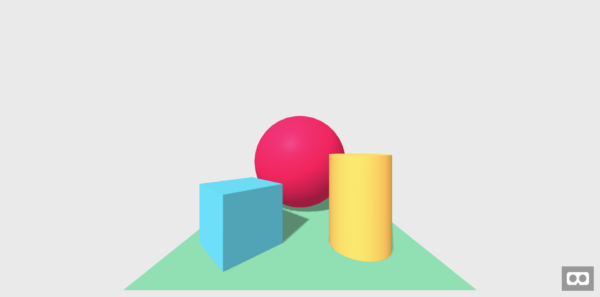
\includegraphics[width=0.7\textwidth]{img/aframe_hello_world.png}
  \caption{Escena básica de A-Frame}
  \label{fig:aframe-basic}
\end{figure}

Una de las principales características de esta tecnología es su arquitectura basada en un modelo de entidad-componente (\textit{Entity Component System}), donde cada objeto dentro de la escena es una entidad que luego es integrada con Three.js para crear la escena.
Una entidad en A-Frame es un objeto HTML que se crea añadiendo la etiqueta \texttt{<a-entity>} y el componente es la apariencia, comportamiento y funcionalidad que se le asigna mediante JavaScript. 

Para hacer uso de un componente se requiere de una serie de pasos previos. Si el componente es externo, es necesario importarlo en la cabecera del HTML, del mismo modo que se importa A-Frame y posteriormente añadirlo a la entidad en la que uno desee usarlo.
Por otra parte, si el componente es de nuestra creación, primero hay que registrar y definir el componente. Esto se hace en un archivo externo de JavaScript mediante el método de \texttt{A-Frame.registerComponente}. A este método, del mimo modo que una función primero se le asigna un nombre, 
este será el nombre del componente. Luego, este método consta de varias funciones internas, las cuales se encargan de definir la apariencia y lógica de dicho componente. Alguna de estas funciones son la función \texttt{schema}, \texttt{init} o \texttt{tick}.
La función \texttt{schema}, define las propiedades principales del componente, estas se pueden modificar dependiendo de la lógica del componente desde el HTML a la hora de llamarlo. La función \texttt{init} se ejecuta una única vez al inicio cuando se inicializa el componente y la función \texttt{tick} se ejecuta a cada frame de la escena.
Una vez el componente está registrado y programado, importamos el archivo que contiene el componente al HTML y lo insertamos a la escena en la entidad u objeto que deseemos. 

Un ejemplo de la llamada de un componente dentro de un archivo de HTML se puede apreciar en \ref{lst:aframe-entity}
\begin{lstlisting}[caption=Ejemplo de llamada de entidad, captionpos=b, label=lst:aframe-entity]
  <html>
    <head>
      <script src="https://aframe.io/releases/1.6.0/aframe.min.js"></script>
      <script src = "componente1.js"></script>
      <script src = "componente2.js"></script>
    </head>
    <body>
      <a-scene>
        <a-entity componente1></a-entity>
        <a-box componente2></a-box>
      </a-scene>
    </body>
  </html>
\end{lstlisting}

En este ejemplo primero se muestra como a una entidad vacía se le añade un componente llamado \texttt{componente 1} y también se muestra como a una entidad de cubo se le añade el componente \texttt{componente 2}.
Del mismo modo, para la creación de un componente, en el archivo \texttt{.js} que posteriormente importaremos en la escena, únicamente es necesario registrar el componente y definir sus características como en el siguiente ejemplo:

\begin{lstlisting}[caption=Ejemplo de creacion de entidad, captionpos=b, label=lst:aframe-entity-creation]
  AFRAME.registerComponent('componente1', {
  init() {
    const box = document.createElement('a-box');
    box.setAttribute('position', '-1 0.5 -3');
    box.setAttribute('rotation', '0 45 0');
    box.setAttribute('color', '#4CC3D9');

    const sphere = document.createElement('a-sphere');
    sphere.setAttribute('position', '0 1.25 -5');
    sphere.setAttribute('radius', '1.25');
    sphere.setAttribute('color', '#EF2D5E');

    this.el.appendChild(box);
    this.el.appendChild(sphere);
  }
});
\end{lstlisting}

Este fragmento de código registra el componente \texttt{componente 1} el cual crea un cubo y un cilindro con unos colores, posición y rotación específicos y los añade a la escena.

Para este proyecto, A-Frame ha sido la tecnología principal, permitiendo elementos fundamentales como la creación y gestión de entornos de realidad virtual. 
También, permitió la integración de componentes diseñados mediante JavaScript y permitió el manejo de interacciones más complejas a la vez que optimizaba el rendimiento de la escena 3D.
\subsection{HTML5}
\label{subsec:HTML5}

HTML5 \cite{freeman2018head} es la quinta iteración del lenguaje de HTML (\textit{marcado de hipertexto}), el cual es la estructura básica y principal de toda página web.
Desarrollado conjuntamente por W3C (\textit{World Wide Web Consortium}) \cite{w3c_mission} y WHATWG (\textit{Web Hypertext Application Technology Working Group}) \cite{whatwg}.
HTML5 introduce mejoras sustanciales respecto a sus anteriores versiones, incluyendo nuevas etiquetas semánticas, soporte multimedia mejorado y compatibilidad
ampliada con diversos navegadores y dispositivos, dándole mayor flexibilidad y dinamismo a la creación de páginas web.

Una de sus nuevas introducciones clave es la introducción de etiquetas semánticas como: \texttt{<header>}, \texttt{<article>}, \texttt{<section>} y \texttt{<footer>},
que facilitan una estructuración clara y accesible del contenido web. Estas etiquetas no solo ayudan a mejorar la organización de la información, sino que también facilitan la búsqueda
de información por parte de los motores de búsqueda y facilitan la interpretación por parte de los desarrolladores.
Además, HTML5 incorpora nuevas interfaces de programación de aplicaciones (\textit{API}), destacándose las funcionalidades de almacenamiento local mediante
\texttt{localStorage} y \texttt{sessionStorage}, que permiten la gestión eficiente de datos directamente en el navegador, eliminando la necesidad de bases de datos externas.

HTML5 también introduce mejoras significativas en la gestión de contenido multimedia, eliminando la necesidad de complementos externos. Para esto se implementaron
las etiquetas \texttt{<audio>} y \texttt{<video>} las cuales permiten la incorporación directa de archivos de sonido y video en las páginas web, permitiendo mayor dinamismo en el desarrollo.
Otro elemento que se añadió fue el elemento \texttt{<canvas>} el cual habilita la generación de gráficos y animaciones en tiempo real a través de JavaScript, permitiendo el desarrollo de aplicaciones interactivas y videojuegos en línea.

HTML5 se ha establecido firmemente como un estándar en el desarrollo de aplicaciones web progresivas (\textit{PWA}) y en entornos multiplataforma. Su integración con tecnologías como CSS3 y JavaScript
permite la creación de interfaces dinámicas y adaptativas, compatibles con una amplia gama de dispositivos, desde ordenadores hasta tabletas y teléfonos.

Gracias a que HTML es una tecnología extensible, tecnologías como A-Frame o WebXR han sido posibles de utilizar, ya que son extensiones de HTML. WebXR permitió poder trabajar con entornos VR desde el navegador, mientras que A-Frame fue el eje central 
del proyecto, donde se estructuró la escena. HTML fue una de las tecnologías más importantes, puesto que ofrece una estructura esencial para el desarrollo del proyecto, haciendo uso de sus extensiones de A-Frame y WebXR para poder mostrar los elementos de la escena en la realidad virtual.

\subsection{JavaScript}
\label{subsec:JavaScript}
JavaScript es un lenguaje de programación ligero y multiplataforma utilizado principalmente para la creación de contenido dinámico e interactivo para páginas web.
Su flexibilidad permite desarrollar elementos para mejorar la interacción del usuario en páginas web tanto del lado del servidor como del lado del cliente. En 1997, JavaScript fue estandarizado
por \textit{ECMA} como ECMAScript y poco después como un estándar \textit{ISO}.

JavaScript, creado por Brendan Eich de Netscape en 1995 bajo el nombre de \textit{Mocha}, posteriormente se renombró a LiveScript y finalmente a JavaScript.
En el año 2000, JavaScript se extendió al lado de los servidores con la introducción de tecnologías como \textit{Node.js}, y posteriormente su popularidad creció con la llegada de \textit{AJAX}. Y Con la llegada de ECMAScript 6 en 2015, se introdujeron características más avanzadas y
actualizaciones anuales, haciendo que hoy en día sea uno de los lenguajes más importantes en el desarrollo web.

JavaScript es un lenguaje de programación de alto nivel, lo que significa que su lenguaje está diseñado para ser lo más 'humano' posible, permitiendo una rápida comprensión del código sin necesidad de un nivel alto de conocimientos.
Es un lenguaje basado en eventos, ya sean entradas de ratón o entradas de teclado, permitiendo la creación de interfaces de usuario interactivas. JavaScript puede integrarse en un HTML dentro de la etiqueta \texttt{<script>} de forma directa, escribiendo el código.
También, se puede introducir códigos de JavaScript, los cuales estén en archivos distintos con la extensión correspondiente al lenguaje (.js), esto es posible vinculando dicho archivo en la cabecera del HTML.

Para este proyecto formo un papel crucial, ya que fue con JavaScript que se desarrollaron los distintos componentes de A-Frame que se usaron para el funcionamiento del proyecto. Permitió diseñar e implementar la lógica que hay tras cada componente, permitiendo alcanzar los resultados obtenidos.

\subsection{Three.js}
\label{subsec:Threejs}

Three.js \cite{webdev_three_intro} es una biblioteca de código abierto de JavaScript utilizada para la creación de gráficos 3D en los navegadores web. Three.js funciona sobre WebGL, la cual permite generar y visualizar animaciones y escenas 3D en el navegador sin necesidad de complementos. La tecnología de WebGL también puede usarse junto con el elemento \texttt{<canva>} de HTML.

Esta biblioteca proporciona una API de alto nivel la cual permite al usuario la creación y manipulación de geometrías 3D como cubos, esfera o planos, así como la aplicación de texturas o la aplicación de tanto cámaras como de efectos de iluminación en las escenas, permitiendo que el desarrollo de dichas escenas sea mucho más simplificado. 
También, Three.js permite la posibilidad de importar modelos 3D desde archivos distintos creados desde aplicaciones distintas.

La biblioteca de Three.js ofrece una alta variedad de herramientas que permiten la gestión y control de usuario, facilitando así tanto la navegación como la interacción dentro de las escenas 3D. También, Three.js soporta animaciones suaves y dinámicas tanto para objetos en la escena como para cámaras, lo cual permite la creación de efectos visuales más dinámicos e impresionantes, al igual que juegos interactivos. 

Gracias a la amplia variedad de posibilidades que permite la biblioteca de Three.js, las opciones de los elementos o escenas que se pueden llegar a crear son básicamente ilimitadas. Siendo capaz de generar escenas complejas como la de la figura \ref{fig:three}
\begin{figure}[H] 
  \centering
  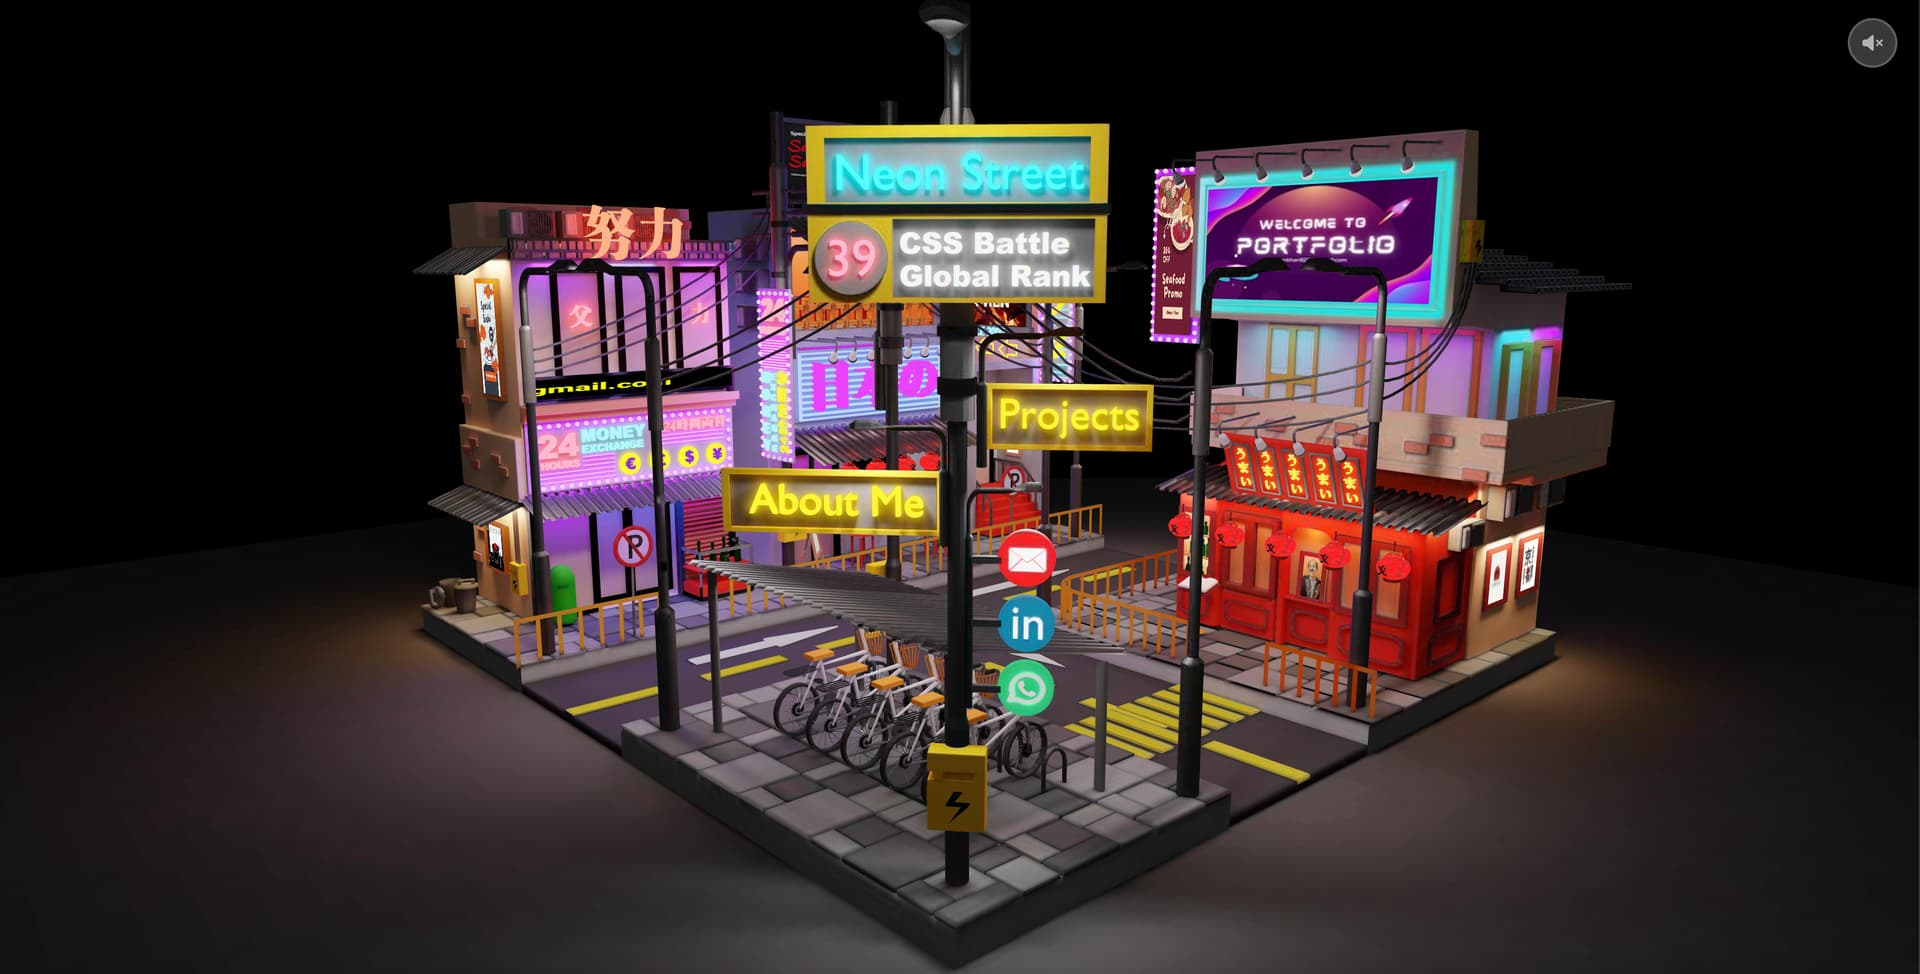
\includegraphics[width=0.7\textwidth]{img/three.jpeg}
  \caption{Escena de Three.js}
  \label{fig:three}
\end{figure}

Three.js permitió añadir una capa más simplificada a WebGL, simplificando así el proceso de creación y manipulación de los elementos 3D. Permitió crear un entorno 3D con mayor dinamismo y control para el proyecto.

\subsection{WebXR}
\label{subsec:WebXR}

WebXR \cite{onirix2024} es una tecnología desarrollada por W3C (\textit{World Wide Web Consortium}) que permite crear experiencias inmersivas desde el navegador. Esta tecnología combina la Realidad Aumentada (\textit{AR}) y la Realidad Virtual (\textit{VR}) con la accesibilidad de un navegador web.
Lo cual permite a los usuarios experimentar e interactuar con entornos tridimensionales a través de cualquier dispositivo con acceso a un navegador compatible.

A medida que la tecnología de WebXR ha ido evolucionando, se han desarrollado distintos tipos de experiencias para poder adaptarse a distintos contextos y necesidades. Hoy en día, se podría clasificar los distintos tipos en 3 categorías:
\begin{itemize}
  \item \textbf{WebXR AR:} Este tipo de WebXR combina el mundo virtual y el mundo real, permitiendo que distintos elementos del mundo virtual puedan superponerse en el entorno físico a través
        de la cámara de un dispositivo compatible, pero sin que llegue a influir el mundo real en los elementos virtuales.
  \item \textbf{WebXR VR:} Este modo permite a los usuarios sumergirse en el entorno virtual creado, y con la ayuda de dispositivos suplementarios como auriculares, la experiencia es aún mayor. Esta tecnología permite a los usuarios
        interactuar y experimentar en primera persona distintos entornos virtuales, desde juegos y entretenimiento, hasta simulaciones virtuales y visualizaciones en 3D.
  \item \textbf{WebXR MR(Mixed Reality):} Esta tecnología combina el mundo real y el virtual de forma más profunda que la tecnología AR. Permite a los usuarios poder interactuar con elementos tantos virtuales como físicos y que estos puedan interactuar entre sí. Este tipo de combinación proporciona un nivel mayor de interacción entre el usuario y
        y su entorno, dando mayor número de posibilidades para la creación de contenido.
\end{itemize}

Estos distintos tipos de WebXR ofrecen distintos tipos de experiencias dependiendo del entorno virtual que se quiera diseñar.

Fue gracias a WebXR, en este proyecto se pudieron realizar las distintas escenas inmersivas que permitieron ir comprobando el avance del proyecto con cada una de las demos que se creaban y que posteriormente se explicaran. Además de eso, fue gracias a WebXR que se pudo realizar la detección de las manos, ya que ya posee una función integrada que permite el handtracking y al querer trabajar sobre el navegador era la mejor opción para ello. 

\subsection{WebGL}
\label{subsec:WebGL}
WebGL \cite{webgl_encodebiz} (\textit{Web graphics Library}), se trata de una tecnología de bajo nivel multiplataforma usada para la renderización de gráficos tanto tridimensionales como bidimensionales dentro de cualquier navegador que sea compatible.

WebGL fue lanzado en 2011 por el grupo Khronos. Esta tecnología se fundamenta en OpenGL ES, la cual es una variante simplificada de OpenGL, diseñada para dispositivos móviles. WebGL ha sufrido numerables actualizaciones, 
lo cual ha permitido una evolución continua que ha ido mejorando tanto su funcionalidad como compatibilidad tanto en navegadores de escritorio como en navegadores en dispositivos móviles. 

WebGL está diseñado para trabajar directamente con la GPU (\textit{Graphic Processing Unit}) del dispositivo, lo cual permite un mayor aprovechamiento de la computación para poder generar gráficos detallados y de alta calidad. 
Además, la tecnología de WebGL está diseñada para poder integrarse de manera fluida con otros estándares de desarrollo web como HTML, CSS o DOM. 

Gracias a esta tecnología fue posible renderizar en la escena las distintas entidades que forman las manos del mismo modo que las otras entidades que se crearon para ir comprobando si los componentes creados funcionaban.

\section{Tecnologias auxiliares}
\label{sec:tecnologias-auxiliares}
En esta sección se detallan y describen las distintas tecnologías que, aunque no hayan influido de manera directa en los resultados del proyecto, han tenido un papel crucial para el desarrollo de este.
Entre dichas tecnologías se encuentra el \textit{IDE} utilizado durante el proyecto, al igual que el dispositivo utilizado para realizar las pruebas de las demos, la plataforma donde se almacenó el código y también el software utilizado para la redacción de esta memoria.

\subsection{Visual Studio Code}
\label{subsec: visualstudiocode}

Visual Studio Code (\textit{VS Code}) es un potente entorno de desarrollo integrado (\textit{IDE}) el cual está disponible para Windows, Linux, MacOS y versión web. VS Code es una de las plataformas de edición de código más utilizadas a nivel mundial 
por toda clase de desarrolladores de software debido a su versatilidad, flexibilidad y amplia gama de extensiones que facilitan la edición y depuración de código.

Una de las pestañas más importantes durante el desarrollo fue su pestaña de \textbf{Source Control}, la cual luego de conectar mi repositorio de GitHub, permite ir guardando el código en GitHub para tener un control de las distintas versiones del código. 

Gracias a las numerosas extensiones que hay disponibles, facilitan en gran medida la creación y depuración de código, permitiendo cosas como autocompletar palabras o expresiones o permitir compilar o depurar con algún lenguaje que VS Code no tenga por defecto.
Algunas de las extensiones utilizadas en este proyecto han sido: 
\begin{itemize}
  \item \textbf{A-Frame completition}: Permite autocompletar rápidamente a la hora de escribir los distintos elementos o Snippets que posee A-Frame
  \item \textbf{Error lens}: A la hora de depuración, permite visualizar dentro del código si hay algún error de sintaxis o lógica 
  \item \textbf{LaTeX Workshop}: Permite la escritura, compilación y previsualización de la memoria de este proyecto.
\end{itemize}

\subsection{GitHub}
\label{subsect:github}

GitHub es una plataforma basada en la nube que permite almacenar distintos repositorios y en cada repositorio código. GitHub está basado en Git \cite{git}, el cual fue creado en 2005 por Linus Torvalds como un sistema de control de versiones de código abierto.
Este sistema fue desarrollado con la intención de ayudar a los desarrolladores a tener en cualquier dispositivo con acceso a internet todo el historial de código que están desarrollando. 

Esta tecnología es ampliamente utilizada a nivel mundial por desarrolladores de todo tipo debido a su capacidad de almacenar, soportar y gestionar proyectos de toda clase. Una de las funciones clave que presenta la plataforma, es la capacidad de crear ramificaciones (branches). Esta opción permite a los desarrolladores poder generar copias del código del repositorio en el que 
están trabajando para poder trabajar en paralelo y posteriormente poder integrar los cambios realizados en paralelo al código principal. Esta opción también permite que más de un desarrollador pueda trabajar en el mismo código, haciendo que cada uno trabaje en paralelo en ramas distintas. 

GitHub aprovecha todas las ventajas que permite Git, permitiendo crear repositorios en la nube para sus proyectos Git, que los desarrolladores pueden llegar a compartir con otras personas. Esta plataforma también facilita la colaboración entre desarrolladores y aparte de las ventajas ya mencionadas de Git permite también el uso de herramientas de gestión de proyectos, al igual que acciones automáticas. 

Durante este proyecto se creó el repositorio de GitHub \textit{TFG}\footnote{\url{https://github.com/JuJoarias/TFG}} donde se fue guardando todas las versiones del código al igual que todas las demos y pruebas realizadas.

\subsection{Meta Quest 3}
\label{subsec:metaquest}

Meta Quest se trata de un dispositivo inalámbrico diseñado para disfrutar de contenido de realidad virtual (VR) por Meta \cite{meta_company_info}. Dicho dispositivo está compuesto por unas gafas, un micrófono y auriculares integrados en un único dispositivo que el usuario pone en su cabeza y un par de mandos inalámbricos. 
La primera versión fue lanzada en 2020 con las Meta Quest 2 y 3 años más tarde, en 2023, se lanzaron las Meta Quest 3. 

Para este proyecto se han utilizado unas Meta Quest 3, las cuales contaban con una memoria de 8 GBB de memoria RAM, una resolución de 2064x2208 píxeles por cada uno de los ojos. También, cuenta con mejoras respecto al campo de visión (FOV) respecto a su versión anterior. Para este proyecto jugaron un papel crucial, ya que al enfocarse en la detección de mandos
el proyecto, sin las gafas, no se habría podido probar los resultados que se iban obteniendo.

\begin{figure}[H] 
  \centering
  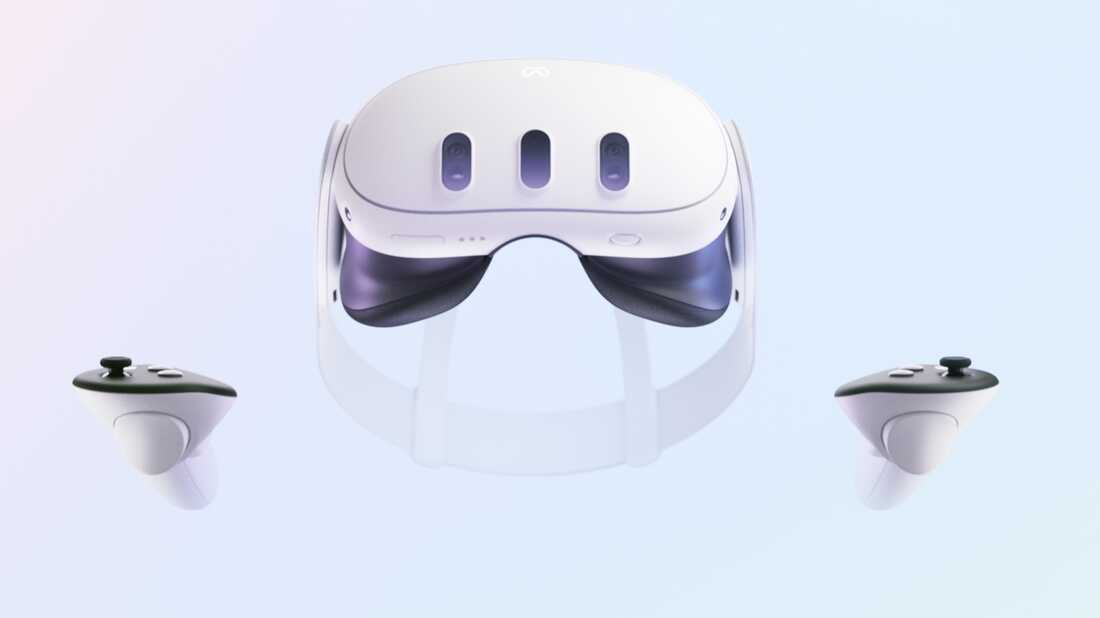
\includegraphics[width=0.7\textwidth]{img/meta_quest.jpg}
  \caption{Meta Quest 3}
  \label{fig:metaquest}
\end{figure}

\subsection{LaTeX}
\label{subsec:latex}

LaTeX \cite{latexproject_about} es un software de uso libre de creación de documentación de alta calidad. Este sistema es altamente utilizado para la creación de documentación técnica o científica de media o larga extensión, aunque gracias a su versatilidad se puede utilizar para cualquier tipo de documentación.

Entre las distintas características de LaTeX cabe destacar su capacidad de manejar expresiones matemáticas complejas, lo cual es una herramienta indispensable para cualquier documento científico. También gracias a su software motor TeX LaTeX es capaz de convertir los comandos de texto, utilizados para expresar los resultados tipográficos, en un archivo PDF profesional. 

Además de facilitar la creación de fórmulas matemáticas complejas, LaTeX también ofrece otras facilidades avanzadas, como puede ser la creación de un índice del contenido, un índice de las figuras utilizadas, gestión de bibliografías o referencias simplificando la organización del documento y la citación de figuras o elementos externos en la bibliografía.

Para este proyecto, LaTeX facilito considerablemente el trabajo a la hora de crear este documento, ayudando con la creación y gestión de índices, imágenes y bibliografía al igual que a estructurar el texto del documento de forma correcta.

%%%%%%%%%%%%%%%%%%%%%%%%%%%%%%%%%%%%%%%%%%%%%%%%%%%%%%%%%%%%%%%%%%%%%%%%%%%%%%%%
%%%%%%%%%%%%%%%%%%%%%%%%%%%%%%%%%%%%%%%%%%%%%%%%%%%%%%%%%%%%%%%%%%%%%%%%%%%%%%%%
% {Desarrollo del proyecto copitulo 3 %
%%%%%%%%%%%%%%%%%%%%%%%%%%%%%%%%%%%%%%%%%%%%%%%%%%%%%%%%%%%%%%%%%%%%%%%%%%%%%%%%

\cleardoublepage
\chapter{Desarrollo del proyecto}
\label{chap:Desarrollo del proyecto}
En este capítulo se describe de forma detallada como fue el desarrollo del proyecto. Dicho desarrollo
se describe en forma de sprints siguiendo una estructura de una metodología \textit{Agile}\cite{asana_agile_methodology}, pese a que el propio proyecto no siguio dicha metodología. 
El desarrollo explica desde los inicios y planteamiento del proyecto hasta obtener los resultados finales.

Por la forma en la que se fue planteando el proyecto, al final de cada sprint se planteaban los objetivos del siguiente para llegar al objetivo final de tener un handtracking funcional y que permitiese interactuar con la escena. 
\section{Sprint 0}
\label{sec:sprint0}
Puesta en marcha del proyecto, planteamiento con el tutor y dominio del uso basico de A-Frame.
\subsection{Objetivos}
\label{subsec:objetivo-principal0}
El objetivo principal de este sprint se puede dividir en 2 partes principales. 
\begin{itemize}
  \item \textbf{Dominio del uso basico de A-Frame}. Aprender a usar de forma correcta como funcionan las escenas al igual que la creación e implementacion de componentes o el uso de librerias de A-Frame.
  \item \textbf{El planteamiento con el tutor}, donde se identificaron las necesidades para el proyecto, también se plantearon los primeros objetivos principales del proyecto, detectar y dibujar las manos y poder usarlas para interactuar con ellas. 
\end{itemize}

\subsection{Tareas Realizadas}
\label{subsec:implementacion0}
La identificación de las necesidades y requisitos de un proyecto es una parte fundamental. Durante las primeras charlas con el tutor se plantearon algunos de los posibles objetivos a los que se podia llegar y los posibles caminos que puede tomar este proyecto. 
Al principio se plantearon varios caminos, pero la idea general de todos ellos era la creación de un sistema de handtracking que sea capaz de interactuar con distintos elementos dentro de la escena. 

Para lograr llegar a ese objetivo primero fue necesario dominar los elementos basicos de A-Frame como biene a ser la organización de la escena, el uso y creación de componentes y el uso de eventos. 
Para ello, primero se creo primero el repositorio de \textit{Git}  con el que trabajaremos durante todo el proyecto. Se crearon una serie de escenas sencillas con el objetivo de dominar el uso de componentes y eventos simples. 
\subsection{Resultados}
\label{subsec:resultados0}
Para familiarimarme aun mas con el entorno de A-Frame se crearon una serie de escenas muy sencillas donde se creaba y utilizaba un componente customizado y se hacia uso del evento nativo de A-Frame \texttt{click}. Estas escenas permitieron un mayor entendimiento del funcionamiento tanto de componentes como de eventos, que fueron fundamentales para el resto del proyecto.
El resultado de dichas pruebas para mejorar la comprensión de A-Frame se pueden apreciar en las figura \ref{fig:sprint0}.
\begin{figure}[H] 
  \centering
  %   \includegraphics[width=0.7\textwidth]{img/...} imagen de la primera escena de test que hice
  \fbox{\rule{0pt}{150pt} \rule{0.7\textwidth}{0pt}} 
  \caption{Escena de test de A-Frame}
  \label{fig:sprint0}
\end{figure}

Tras la familiarización con el entorno de A-Frame y sus características el proyecto fue formalizado formalmente. Tras ellos se planteo el siguiente sprint del proyecto donde ya se empezarian los primeros pasos formales de este. 

\section{Sprint 1}
\label{sec:sprint1}
Investigación del handtracking y primeras implementaciones de este en el proyecto.

\subsection{Objetivos}
\label{subsec:objetivo-principal1}
En este primer sprint oficial del proyecto, el objetivo princpial era investigar y comprender el uso del handtracking en A-Frame. 
Este era el paso principal en el que se basaria todo el proyecto, ya que sin una comprensión del funcionamiento del handtracking en A-Frame este proyecto habria sido imposible de realizar.
Además de obtener una primera demo del handtracking en la escena.
\subsection{Tareas Realizadas}
\label{subsec:implementacion1}
Los primeros pasos fue investigar el handtracking en A-Frame con los elementos ya existentes como \textit{\texttt{super hands}}\footnote{\url{https://github.com/c-frame/aframe-super-hands-component}}, o los componentes nativos de A-Frame \texttt{hand-controls} o \texttt{hand-tracking-controls}.
Para ellos se usaron pequeñas escenas de prueba para comprender mejor el comportamiento de las manos en la realidad virtual, y del mismo modo, tener una idea mas clara del objetivo final del aspecto de handtracking. 

Tras la investigación de las manos y la sugerencia del tutor, se decidio utilizar la tecnologia de WebXR para el handtracking puesto que esta tecnología ya posee un sistema preparado para ello. Además, usando la tecnología de WebXR nos permitia trabajar con cada una de las articulaciones de la mano de forma independiente. 

Siguiendo la documentación de \textit{WebXR}\footnote{\url{https://www.w3.org/TR/webxr-hand-input-1/}}, se empezo el desarrollo de las manos. para ello en el codigo fue necesario tratar cada una de las manos de forma independiente, del mismo modo que cada una de las articulaciones como se muestra en el esquema de las manos de WebXR en la figura \ref{fig:WebXR-manos}. 

\begin{figure}[H] 
  \centering
  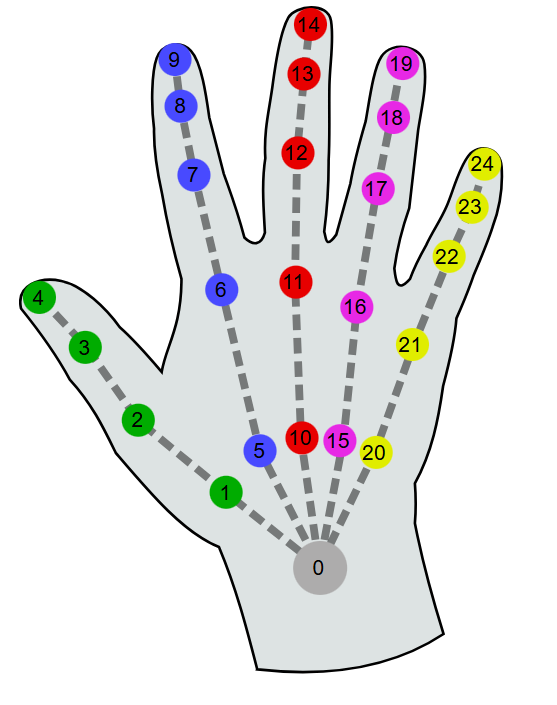
\includegraphics[width=0.4\textwidth]{img/webxr-mano.png} 
  \caption{Esquema manos segun WebXR}
  \label{fig:WebXR-manos}
\end{figure}

Para poder crear las manos de forma exitosa dentro del entorno de realidad virtual siguiendo WebXR, primero se crea el componente que sera el encargado de detectar y dibujar las manos en este proyecto, dicho componente se llama \texttt{hand-skeleton}. Dicho componente no tenia un \texttt{schema}, en el \texttt{init} se definian las distintas variables que eran necesarias para el funcionamiento del código. 
En el HTML que define la escena unicamente era necesario añadir una vez el componente como una entidad. Pero era imprescindible definir todas y cada una de las articulaciones, como se muestra en el fragmento de código \ref{lst:articulaciones}, pero esa definición unicamente se realizaba en el código de JavaScript.
\begin{lstlisting}[caption=Definición de articulaciones, captionpos=b, label=lst:articulaciones]
  const orderedJoints = [
    ["wrist"],
    ["thumb-metacarpal", "thumb-phalanx-proximal", "thumb-phalanx-distal", "thumb-tip"],
    ["index-finger-metacarpal", "index-finger-phalanx-proximal", "index-finger-phalanx-intermediate", "index-finger-phalanx-distal", "index-finger-tip"],
    ["middle-finger-metacarpal", "middle-finger-phalanx-proximal", "middle-finger-phalanx-intermediate", "middle-finger-phalanx-distal", "middle-finger-tip"],
    ["ring-finger-metacarpal", "ring-finger-phalanx-proximal", "ring-finger-phalanx-intermediate", "ring-finger-phalanx-distal", "ring-finger-tip"],
    ["pinky-finger-metacarpal", "pinky-finger-phalanx-proximal", "pinky-finger-phalanx-intermediate", "pinky-finger-phalanx-distal", "pinky-finger-tip"]
  ];
\end{lstlisting}
Después de definir todas las articulaciones era necesario procesarlas. 
Para ello, se creo la función que se muestra en el fragmento de código \ref{lst:manos-codigo}. En la función \texttt{renderHandSkeleton} se crea un bucle de código el cual, toma la sesión XR de la escena y por cada input de la sesion toma cada una de las articulaciones, las detecta en la mano y crea una esfera a traves de una segunda función unicamente encargada de crear esferas. Dichas esferas se crean en la posición corerspoondiente a la mano real
y tambien se ajusta el radio de la esfera para que coincida con la mano. 

\begin{lstlisting}[caption=Dibujo de las manos en la escena, captionpos=b, label=lst:manos-codigo]
  renderHandSkeleton: function () {
    const session = this.el.sceneEl.renderer.xr.getSession();
    if (!session || !this.frame || !this.referenceSpace) {
        return;
    }
    const inputSources = session.inputSources;
    for (const inputSource of inputSources) {
        if (inputSource.hand) {
            const hand = inputSource.hand;
            const handedness = inputSource.handedness; // Determina si es la mano derecha o izquierda
            for (const finger of orderedJoints) {
                for (const jointName of finger) {
                    const joint = hand.get(jointName);
                    if (joint) {
                        const jointPose = this.frame.getJointPose(joint, this.referenceSpace);
                        if (jointPose) {
                            const position = jointPose.transform.position;
                            if (!this.spheres[handedness + '_' + jointName]) {
                                this.spheres[handedness + '_' + jointName] = this.drawSphere(jointPose.radius, position);
                            } else {
                                this.spheres[handedness + '_' + jointName].object3D.position.set(position.x, position.y, position.z);
                            }
                        }
                    }
                }
            }
        }
    }
  },
\end{lstlisting}

Esta función se encuentra dentro de la función \texttt{tick} del componente manos, asi que a cada frame el propio código revisa la posición de todas y cada una de las articulaciones para cada una 
de las dos manos de entrada.
Además de detectar y dibujar las manos en la escena, en esta primera demo se implementó el gesto de \texttt{Pinch}, distinguiendo cada mano y realizando una acción distinta dependiendo de la mano que lo realizase. 

Primero, para la detección del gesto se creo la función de \texttt{detectGestures}, como se muestra en el fragmento de código \ref{lst:firstdetectGesture}. En dicha función, se tomaba la posición del la punta del dedo índice y del pulgar y se calculaba la distancia entre ambos puntos.

\begin{lstlisting}[caption=Función detectGestures, captionpos=b, label=lst:firstdetectGesture]
  detectGestures: function () {
    const session = this.el.sceneEl.renderer.xr.getSession();
    const inputSources = session.inputSources;
    let rightPinching = false;
    let leftPinching = false;
    for (const inputSource of inputSources) {
        if (inputSource.hand) {
            const thumbTip = this.frame.getJointPose(inputSource.hand.get("thumb-tip"), this.referenceSpace);
            const indexTip = this.frame.getJointPose(inputSource.hand.get("index-finger-tip"), this.referenceSpace);
            if (thumbTip && indexTip) {
                const distance = calculateDistance(thumbTip.transform.position, indexTip.transform.position);
                if (distance < pinchDistance) {
                    if (inputSource.handedness === 'right') {
                        rightPinching = true;
                        if (!this.rightPinching) {
                          this.createBoxAtHand(inputSource.hand);  
                        }
                    } else if (inputSource.handedness === 'left') {
                        leftPinching = true;
                        if (!this.leftPinching) {
                            this.selectObjectAtHand(inputSource.hand); // Selecciona un objeto cercano para mover
                        }
                    }
                }
            }
        }
    }
    this.rightPinching = rightPinching;
    this.leftPinching = leftPinching;
  },
\end{lstlisting}

Si la distancia era inferior a 0.02 (valor obtenido tras realizar varias pruebas), se comprobaba que mano era la que lo realizaba y luego se llamaba a la función correspondiente. 
Si se trataba de la mano derecha, se creaba un cubo verde en la posición de la punta del dedo índice. Y si se trataba de la mano izquierda, si esta se encontraba lo bastante cerda de uno de los cubos creados por la mano derecha (a una distancia inferior a 0.15) la posición del cubo copiaria la de la punta del dedo índice izquierdo hasta que se soltase el gesto.


\subsection{Resultados}
\label{subsec:resultados1}

Como resultado de este sprint se creo la demo de \textit{pinch test}\footnote{\url{https://github.com/JuJoarias/TFG/blob/main/first_steps/first_hands/pinch_test.html}} al igual que en la figura \ref{fig:sprint1}.

\begin{figure}[H] 
  \centering
  %   \includegraphics[width=0.7\textwidth]{img/...} imagen de la primera escena de manos
  \fbox{\rule{0pt}{150pt} \rule{0.7\textwidth}{0pt}} 
  \caption{Primera demo de manos}
  \label{fig:sprint1}
\end{figure}

Las esferas se dibujaban correctamente y los gestos funcionaban, pero habia bastantes aspectos a mejorar. Primero, por sujerencia del tutor,
se debia modificar el componente para que fuese necesario añadirlo 2 veces a la escena, 1 por cada mano. También, respecto al gesto, con la mano derecha habia que cambiar el funcionamiento
ya que el que creara un cubo no seria necesario mas adelante. Y respecto a la mano izquierda, se identificó que a la hora de tomar el cubo, este se transportaba hacia la posicion del dedo índice. 
Y aunque esto era lo deseado de primeras, visualmente no quedaba bien ya que si se agarraba una esquina el cubo se transportaba, tragandose la mano en vez de agarrar el cubo mientras mantenia la distance entre el dedo y el centro del cubo. 
Aparte de eso, en el caso de que hubiese mas de un cubo muy pegado, el código no identificaba siempre de forma correcta el mas cercano, haciendo que a veces se tomara el cubo no deseado.

Todos estos factores dieron paso al siguiente sprint, donde se corregirian los errores resaltados. Aparte se intentaria optimmizar la creación de las manos y se añadiria la emisión y gestión de eventos, ya que en esta primera demo, al realizar el gesto, se llama a la función correspondiente si utilizar eventos. 

\section{Sprint 2}
\label{sec:sprint2}
Introducción de eventos y optimización del manejo de manos. 

\subsection{Objetivos}
\label{subsec:objetivo-principal2}
Tras la observaciones del sprint anterior, para este sprint se replanteo el funcionamiento de los gestos. También, se reorganizo la forma de creación de las manos en la escena y la detección de los gestos. 


\subsection{Tareas Realizadas}
\label{subsec:implementacion2}
Primero, se reorganizo el componente encargado de dibujar las manos que se creo en el sprint anterior. Dicho componente se renombro a \texttt{manos}, nombre que se mantendría hasta el final del proyecto. A dicho componente se le añadio un \texttt{schema}. 
En dicho \texttt{schema} hay unacamente una variable llamada \texttt{hand}, dicha variable unicamente acepta \texttt{left} o \texttt{right} como entradas. Este cambio era para que el componente distinguiera las manos y unicamente dibujase una mano a la vez, esto hizo que para dibujar ambas manos en la escena fuese necesario añadir el componente 2 veces, 1 por cada mano. 
También, se modifico la función \texttt{init}. Ahora, aparte de definir los valores iniciales de las variables utilizadas, realiza un bucle que recorre la constante que contiene todas las articulaciones y por cada una crea una esfera. Dichas esferas son añadidas a la escena y tambien se crea un diccionario al que se le añade el nombre y entidad de cada articulación.
Este bucle se puede apreciar en el fragmento de código \ref{lst:esferas}. Como se puede apreciar, esto no nos permite detectar las manos y utilizarlas en la escena, simplemente prepara las entidades que representaran la mano dentro de la escena.

\begin{lstlisting}[caption=Creación de las esferas de las articulaciones, captionpos=b, label=lst:esferas]
  orderedJoints.flat().forEach((jointName) => {
    const jointEntity = document.createElement('a-sphere');
    jointEntity.setAttribute('color', 'white'); 
    this.el.appendChild(jointEntity);
    this.joints[jointName] = jointEntity;
  });
\end{lstlisting}

Para la actualización de la posición de todas las articulaciones se creao la funcion que se muestra en el fragmetno de código \ref{lst:nuevas_manos}. Esa nueva función es una versión actualizada de la que se creo en el sprint anterior. 
La principal diferencia con el código previo es que este unicamente trabaja con la mano que se definió en el \texttt{schema} y trabaja directamente con las entidades que estan guardadas en el diccionario que se creo en el \texttt{init}. 

\begin{lstlisting}[caption=Actualización de las manos, captionpos=b, label=lst:nuevas_manos]
  updateSkeleton: function () {
    const session = this.el.sceneEl.renderer.xr.getSession();
    const inputSources = session.inputSources;
    for (const inputSource of inputSources) {
      if (inputSource.handedness === this.data.hand && inputSource.hand) {
        for (const [jointName, jointEntity] of Object.entries(this.joints)) {
          const joint = inputSource.hand.get(jointName);
          const jointPose = this.frame.getJointPose(joint, this.referenceSpace);
          
          if (jointPose) {
            const { x, y, z } = jointPose.transform.position;
            const radius = jointPose.radius; 
            jointEntity.setAttribute('position', { x, y, z });
            jointEntity.setAttribute('radius', radius || 0.008);
          } else {
            jointEntity.setAttribute('position', '0 0 0'); // Esconder si no hay datos
          }
        }
      }
    }
  },
\end{lstlisting}

Para la detección del gesto la lógica general permanece igual, pero en vez de llamar a otras funciones se emiten los eventos \texttt{pinchstart} y \texttt{pinchend} dependiendo de si se esta realizando el gesto o no y junto al evento se envia como argumento de este la mano que lo realiza, la derecha u izquierda.

Para escuchar los eventos, se creo el componente \texttt{detector}. Este componente posee 2 variables en su \texttt{schema}. La primera es que mano detectara, del mismo modo que el componente \texttt{manos}, y la segunda es un target. El target es principalmente para debug de la escena, ya que para esta demo se añadieron 2 entidades a la escena las cuales 
eran texto. Asi que el target seria el ID de una de esas entidades de texto.
Este componente cada vez que reciviese un evento se encargaria de modificar el texto del target, señalando si se ha iniciado o terminado el gesto y de que mano. 

\subsection{Resultados}
\label{subsec:resultados2}
El resultado de este sprint fue el código \textit{componentes}\footnote{\url{https://github.com/JuJoarias/TFG/blob/main/first_steps/first_hands/componentes.html}}.

\begin{figure}[H] 
  \centering
  %   \includegraphics[width=0.7\textwidth]{img/...} imagen de la escena de componentes.html
  \fbox{\rule{0pt}{150pt} \rule{0.7\textwidth}{0pt}} 
  \caption{Primera demo de manos}
  \label{fig:sprint2}
\end{figure}

En este sprint a nivel visual en la escena no habia grandes cambios ya que el objetivo principal era la optimización de la creación de las manos y la introducción de los eventos. 
Como se aprecia en la figura \ref{fig:sprint2}, dentro de la escena se dibujan las manos correctamente y los texton se modifican com oes debido. Para esta demo, para los gestos unicamente se implemento el cambio de texto ya que 
como aun no se trabajaba con los gestos y hacia falta añadir mas, se queria una forma mas sencilla de comprobar que los eventos se emitian y escuchaban correctamento. 

\section{Sprint 3}
\label{sec:sprint3}
Nuevos gestos de las manos

\subsection{Objetivos}
\label{subsec:objetivo-principal3}
Para este nuevo sprint, el objetivo principal era introducir mas gestos. Hasta ahora unicamente estaba implementado el gesto de \texttt{Pinch}.
Durante este sprint se planeo introducir la logica de los gestos \texttt{Fist}, \texttt{Point} y \texttt{Openhand}.

\subsection{Tareas Realizadas}
\label{subsec:implementacion3}
Para conseguir implementar los nuevos gestos principalmente hizo falta modificar la función de \texttt{detectGesture}, aparte de eso, para poder distinguir bien que gesto se esta realizando, en el \texttt{init} se definio una variable booleana por cada gesto, las cuales cambian dependiendo de si se esta realizando el gesto o no. Estas variables se implementaron ya que, como la comprobación de los gestos y emisión de estos se realizan en la función \texttt{tick}, si no se implementa esta lógica, se emitiria el mismo evento repetidas veces cuando unicamente es necesaria una vez.

Para ello, primero se buscaba la posicion de la punta de todos los dedos y de la muñeca. Una vez con todas las posiciones obtenidas, mediante una función se calculaba la distancia de la punta del dedo correspondiente a la muñeca y si esa distancia era inferior a 0.09 (obtenido luego de varias pruebas para que sea una distancia optima), se definia que el dedo en cuestion estaba doblado.
Para cada dedo hay una constante booleana que esta True si el dedo esta doblado y false si esta estirado. Ahora con la información de cada dedo se comprueba si estan estirados o no y dependiendo del estado de los dedos y de si la variable de estado de los gestos esta a True o False, se emite el evento start o end correspondiente a cada gesto. 

\subsection{Resultados}
\label{subsec:resultados3}
Como resultado, se obtuvo la demo de \textit{nuevos gestos}\footnote{\url{https://github.com/JuJoarias/TFG/blob/main/first_steps/second_hands/nuevos_gestos.html}}

\begin{figure}[H] 
  \centering
  %   \includegraphics[width=0.7\textwidth]{img/...} imagen de la escena de nuevos gestos
  \fbox{\rule{0pt}{150pt} \rule{0.7\textwidth}{0pt}} 
  \caption{Primera demo de manos}
  \label{fig:sprint3}
\end{figure}

El resultado fue bastante similar al del sprint anterior, pero con la principal diferencia de que se habian añadido mas gestos a la lógica de las manos como se aprecia en la figura \ref{fig:sprint3}

Ahora que teniamos una lógica de detección de manos y de gestos era tiempo de crear la la lógica necesaria para poder interactuar con los elementos dentro de la escena, para lo cual, primero era necesario saber cuando las manos estaban colisionando con los elementos de la escena. 
\section{Sprint 4}
\label{sec:sprint4}
Incorporación de colliders  

\subsection{Objetivos}
\label{subsec:objetivo-principal4}
Como ultimo paso de preparación de las manos era necesario saber cuando las manos estaban interactuado con los elementos de la escena. El objetivo principal de este sprint era la incorporación de Incorporación de colliders  
en la escena. 


\subsection{Tareas Realizadas}
\label{subsec:implementacion4}
Para añadir Incorporación de colliders  
a la escena se hizo uso del componente propio de A-Frame \textit{obb-collider}\footnote{\url{https://aframe.io/docs/1.7.0/components/obb-collider.html}}.
La principal ventaja que nos proporciona el uso de este componente nativo de A-Frame, era que cuando detecta una colisión entre 2 entidades que posean dicho componente este lanza un evento indicando el inicio de la colisión y cuando no hay colisión lanza otro indicando el final de la colisión.
Los eventos que lanza el componente eran \texttt{obbcollisionstarted} y \texttt{obbcollisionended}.

Lo principal para añadir los Incorporación de colliders  
era añadirlos a la mano, ya que añadirlos a los distintos elementos de la escena era tan sencillo como añadir el componente de \texttt{obb-collider}. Para ello,
habia que modificar la función encargada de actualizar las articulaciones de las manos. 

Dentro de la función de \texttt{updateSkeleton} \ref{lst:nuevas_manos} se añade las siguientes lineas de código:

\begin{lstlisting}[caption=Añadir Incorporación de colliders a la mano, captionpos=b, label=lst:colliders]
  
  if (!jointEntity.hasAttribute('obb-collider')) {
    jointEntity.setAttribute('obb-collider', `size: ${radius * 2} ${radius * 2} ${radius * 2}`);
  }
\end{lstlisting}

Como se aprecia en el código \ref{lst:colliders}, se comprueba si la articulación en cuestion tiene ya un colider y si no lo tiene lo añade.

\subsection{Resultados}
\label{subsec:resultados4}
Como resultado de este sprint se obtuvo la demo de \textit{colliders}\footnote{\url{https://github.com/JuJoarias/TFG/blob/main/first_steps/second_hands/colliders.html}}. 

\begin{figure}[H] 
  \centering
  %   \includegraphics[width=0.7\textwidth]{img/...} imagen de la escena de colliders
  \fbox{\rule{0pt}{150pt} \rule{0.7\textwidth}{0pt}} 
  \caption{Primera demo de manos}
  \label{fig:sprint4}
\end{figure}

En dicha escena se mantienen los logros que ya habiamos obtenido en los sprints anteriores. Y para comrpobar el funcionamiento de los colliders se añadio a la escena un cubo
al que le añadimos el componente de \texttt{obb-collider}. En dicha escena se implemento la lógica de que si se detectaba colisión entre el cubo y las manos  el color del cubo cambiaria para tener una respuesta mas visual. 

Mientras se comprobaba el funcionamiento se noto un error. Como la mano estaba formada por varias esferas con espacios entre medias, y cada  esfera poseia un colliders, se emitian varias veces los eventos de inicio y fin de la colisión incluso si no se sacaba la mano del cubo. 
Esto era un problema ya que estos eventos repetidos cuando no corresponden hacian que cualquier función implementada cuando se detecta colisión actue de forma intermitente y por lo tanto erronea. Aunque este problema no fue identificado hasta el sprint siguiente. 

\section{Sprint 5}
\label{sec:sprint5}
Función grabable

\subsection{Objetivos}
\label{subsec:objetivo-principal5}
Para este sprint se quiso ya ir incorporando el funcionamiento de los gestos en la escena. Para empezar se quiso trabajar con el gesto \texttt{Pinch}. Se planteo que si se hacia con la manos derecha sobre el cubo poder 
arrastrar dicho cubo por la escena en cualquier dirección e imitando la rotación de la mano para que parezca que lo estamos agarrando realmente. Y si se hacia con la mano izquierda, el cubo unicamente se podria deslizar en un unico eje, el eje X.

\subsection{Tareas Realizadas}
\label{subsec:implementacion5}
Este sprint fue uno de los mas complejos hasta ahora, ya que a lo largo del proceso fuimos encontrando distintos problemas que hicieron replantear la lógica del código. 

Para empezar con este sprint, se creo el componente de \texttt{Grabable}, dicho componente no posee un \texttt{schema}. Y en su init aparte de definir las distintas variables necesarias, se comprueba si la entidad a la que se añada el componente posee un collider, y en caso de no tener le añade uno.
En este componente toda la lógica se ejecuta dentro la una función llamada \texttt{check}, la cual se llama en el \texttt{tick}. 

En dicha función, lo primero que se compruba es si hay una colisión, y si la hay ocurren 2 procesos importantes. El primero, es que se cambia el estado de una variable booleana la cual indica si hay colisión o no, y el segundo, se ejecuta una función llamada \texttt{hoover}. En esa función para saber de forma visual que estamos interactuando con el cubo, incluso antes de realizar ningun gesto, se cambia la trasparencia del cubo ligeramente.

Luego, para distinguir entre el pinch de la mano derecha y la mano izquierda escuchamos los eventos de \texttt{pinchstart} y \texttt{pinchend} ya que el evento lleva la información de la mano que esta realizando el gesto. Con esa información se cambia la variable boolenan correspondiente para saber que mano realiza el gesto. Una vez con esa información ya se podia realizar la lógica del gesto.

Para poder realizar correctamente la lógica del gesto, era necesario poder acceder a la información de las entidades que forman las articulaciones. Para ello, debiamos de ser capaces de acceder a la información del componente \texttt{manos} mediante las siguientes lineas de código:

\begin{lstlisting}[caption=Acceso información componente manos, captionpos=b, label=lst:info_manos]
  
  this.leftHandEntity = document.querySelector('#left-hand');
  this.rightHandEntity = document.querySelector('#right-hand');

  const manoDerecha = this.rightHandEntity.components.manos;
  const manoIzquierda = this.leftHandEntity.components.manos;
\end{lstlisting}

Con eso ya somos capaces de acceder a la información de \texttt{joints}, donde se almacenaban todas las entidades de las articulaciones.

Para la mano izquierda fue mas sencillo. Se comprobaba si habia solisión con el cubo y tambien si la variable correspondiente al pinch de la mano izquierda estaba en True, y de estarlo, el cubo cambiaba su color a azul y posteriormente se procede a acceder a la información 
de la punta del indice de la mano izquierda y se hace que el cubo copie la coordenada de dicha articulación mientras mantiene sus otras coordenadas, asi se desliza unicamente en un único eje.

Para la manos derecha fue mas complejo. Se queria poder agarrar el cubo y poder deslizarlo y rotarlo a antojo del usuario. Para ello se planteo hacer un \texttt{reparenting}, para volver la entidad del cubo hija de la entidad de la mano para que asi imitara sus movimientos y rotaciones. Para realizar esto se realizo un \textit{test externo}\footnote{\url{https://github.com/JuJoarias/TFG/blob/main/external_tests/reparenting_test.html}}.
El test dio los resultados deseados, pero a la hora de aplicarlo al código resaltaron varios probelmas. 

El primero, era que no se lograba realizar el \texttt{reparenting} con la entidad de la mano, asi que para solucionarlo se obto por que el nuevo padre del cubo fuese la punta del dedo índice mientras se realizaba el gesto.
Otro fallo que resalto fue la rotación. Pese a que el \texttt{reparenting} se realizaba correctamente, el cubo no seguia las rotaciones de la mano. Y esto se debia a como se dibujaban las manos, ya que a cada frame se actualiza la posición de cada articulación, pero no la rotación, con lo cual esta se mantiene fija. Para solucionar este problema, se obto por tomar 3 articulaciones de la mano y con estas 
como referencia para los ejes X y Z se creo un eje de coordenadas relativo. Dicho eje relativo seguiria la orientación y rotación de la mano. Una vez obtenido ese eje cuando se realiza el gesto derecho el cubo empieza a imitar dicho eje, permitiendo que el cubo rote al mismo tiempo que se arrastra el cubo por la escena. 
\subsection{Resultados}
\label{subsec:resultados5}
El resultado de este sprint se refleja en la demo \textit{hands grabable}\footnote{\url{https://github.com/JuJoarias/TFG/blob/main/first_steps/second_hands/hands_grabable.js}}. 

\begin{figure}[H] 
  \centering
  %   \includegraphics[width=0.7\textwidth]{img/...} imagen de la escena de grabable
  \fbox{\rule{0pt}{150pt} \rule{0.7\textwidth}{0pt}} 
  \caption{Manos Grabable}
  \label{fig:sprint5-1}
\end{figure}

\begin{figure}[H] 
  \centering
  %   \includegraphics[width=0.7\textwidth]{img/...} imagen de la escena de grabable
  \fbox{\rule{0pt}{150pt} \rule{0.7\textwidth}{0pt}} 
  \caption{Manos Grabable}
  \label{fig:sprint5-2}
\end{figure}

Como se aprecia en las figuras \ref{fig:sprint5-1} y \ref{fig:sprint5-2} cada vez que se realiza el gesto con cada una de las manos sobre el cubo este reacciona de manera distinta. 
El color cabia para tener una respuesta mas visual además de que cada mano tenia se propia reacción. 

Con esto se habia conseguido implementar las acciones de \texttt{Hoover}, \texttt{Drag} y \texttt{Slide}. De cara al siguiente sprint se decidio organizar mejor el código de dichas acciones al igual que añadir las acciones de \texttt{Stretch} y \texttt{Click}

\section{Sprint 6}
\label{sec:sprint6}
Manos finales

\subsection{Objetivos}
\label{subsec:objetivo-principal6}
El objetivo de este ultimo sprint era añadir nuevas acciones y organizar mejor el código para que quedase lo mas limpio posible. 
También, por sugerencia del tutor se intento modificar el código para que las manos diseñadas en este proyecto funcionasen junto con el componente ya existente de \texttt{Superhands}, aunque esto no se logro al final. 

\subsection{Tareas Realizadas}
\label{subsec:implementacion6}
Para empezar con este sprint, primero se decidio por organizar el código ya existente y las acciones. Para ello, por cada acción que ya estaba implementada , \texttt{Hoover}, \texttt{Drag} y \texttt{Slide}, se creo un componente. También, el componente \texttt{Grabable}, creado en el sprint anterior fue modificado para que en vez de llamar directamente a las funciones encargadas de las acciones de los gestos, emita los eventos \texttt{Start} o \texttt{End} correspondeintes a cada acción. 

Dichos eventos luego serian escuchados por el componente correspondiente. La estructura de los componentes de las acciones todos siguen la misma estructura. En el \texttt{Init} primero se comprueba si la entidad a la que fue añadido contiene también el componente \texttt{Grabable} y si no lo tiene lo añade ya que este componente es indispensable para que los componentes de acciones funcionen a excepción del componente correspondiente al \texttt{Click}. Luego de eso, el componente escucha los eventos de \texttt{Start} y \texttt{End} y si los escucha llama a una función
, la cual inicializa los datos o variables correspondientes que posteriormente se usaran en la función \texttt{Tick} del componente. En el siguiente fragmento de código se aprecia el componente \texttt{hoover} como ejemplo:

\begin{lstlisting}[caption=Componente Hoover, captionpos=b, label=lst:Hoover]
  
  AFRAME.registerComponent('hoover', {

    init: function(){
        if (!this.el.hasAttribute('grabable')) {
            this.el.setAttribute('grabable', '');
        }

       this.el.addEventListener('hooverStart', this.onHooverStart.bind(this));
       this.el.addEventListener('hooverEnd', this.onHooverEnd.bind(this));
       this.hooverState = false;
       this.isHoovering = false;
    },

    onHooverStart: function () {
       if (this.isHoovering) return;
       this.isHoovering = true;

       this.hooverState = true;
    },

    onHooverEnd: function () {
       this.hooverState = false;
       this.isHoovering = false;
    },

    tick: function () {
        if (this.hooverState){
           this.el.setAttribute('material', 'opacity', '0.8');
        } else{
           this.el.setAttribute('material', 'opacity', '1');
        }
    },
});
\end{lstlisting}

Para los componentes de \texttt{Slide} y \texttt{Drag} se ha mantenido la lógica obtenida en el sprint anterior, pero aplicando la estructura mostrada. 
También, al componente \texttt{Slide}, se le añadio un \texttt{Schema}. Este componente es el único que lo tiene y en el se puede definir en que eje queremos que se deslice el objeto, ya no se limita al eje X.

Respecto al componente de \texttt{Stretch}, la lógica detras del gesto es similar a las acciones previamente implementadas. La única diferencia es que este componente unicamente reacciona cuando se esta haciendo el gesto sobre el mismo objeto con ambas manos a la vez.
Una vez activado, el componente comprueba la distancia entre la punta de los dedos indices de ambas manos y con esa distancia la guarda en una variable. Utilizando esa distasncia inicial, se crea un factor de escalado al dividir la distancia actual entre las manos y la inicial. Posteriormente se multiplica dicho factor por la escala del objeto, asi esta crecera o decrecera dependiendo de la distancia entre ambas manos. 

Hasta ahora todas las acciones habian funcionado con el gesto \texttt{Pinch}, pero para la accion de \texttt{Click} era necesario otro. Para este componente se utilizo el gesto de \texttt{Point}, el cual consistia en tener el dedo índice estirado. Al relizar el gesto el código crearía un puntero desde la punta del dedo y a cada frame actualizaria su dirección utilizando como vector la línea que une la punta del dedo con su nudillo. 
Ahora que teniamos el puntero era necesaria una acción para que se emitiera el evento. Para ello, se utilizó el dedo pulgar. Como si se tratase de una pistola, se configuró el código para que cuando se haga el gesto de "disparar una pistola" se emitiera el evento de click. Toda esta implementación del gesto se introdujo directamente dentro del componente principal, el componente \texttt{Manos}. 
Posteriormente, en el propio componente, al escuchar el evento este componente unicamente cambia el color del cubo a morado y al soltar el gesto de pistola, sin necesidad de soltar el gesto de \texttt{Point}, el color vuelve a su color original. 
\subsection{Resultados}
\label{subsec:resultados6}
El resultado de este sprint es la propia \textit{demo}\footnote{\url{https://github.com/JuJoarias/TFG/blob/main/demo/demo.html}} presentada al final. 

\begin{figure}[H] 
  \centering
  %   \includegraphics[width=0.7\textwidth]{img/...} imagen de la escena de grabable
  \fbox{\rule{0pt}{150pt} \rule{0.7\textwidth}{0pt}} 
  \caption{Manos finales 1}
  \label{fig:sprint6-1}
\end{figure}

\begin{figure}[H] 
  \centering
  %   \includegraphics[width=0.7\textwidth]{img/...} imagen de la escena de grabable
  \fbox{\rule{0pt}{150pt} \rule{0.7\textwidth}{0pt}} 
  \caption{Manos finales 2}
  \label{fig:sprint6-2}
\end{figure}

En las figuras \ref{fig:sprint6-1} y \ref{fig:sprint6-2} se muestran algunas de las acciones implementadas durante este proyecto. En esta demo se aprecia un cubo por cada acción que se implemento al igual que un cubo que posee todas ya que cada cubo unicamente cuenta con uno de los componentes de acción.
%%%%%%%%%%%%%%%%%%%%%%%%%%%%%%%%%%%%%%%%%%%%%%%%%%%%%%%%%%%%%%%%%%%%%%%%%%%%%%%%
%%%%%%%%%%%%%%%%%%%%%%%%%%%%%%%%%%%%%%%%%%%%%%%%%%%%%%%%%%%%%%%%%%%%%%%%%%%%%%%%
% RESULTADOS capitulo 4%
%%%%%%%%%%%%%%%%%%%%%%%%%%%%%%%%%%%%%%%%%%%%%%%%%%%%%%%%%%%%%%%%%%%%%%%%%%%%%%%%

\cleardoublepage
\chapter{Resultados}
\label{chap:resultados}
En este capítulo se se describen en detalle los resultados obtenidos a lo largo de este proyecto, así como una descripción funcional de este, donde se desarrollan las partes básicas de la conclusión del proyecto de forma funcional. También, en este capítulo se incluye un manual de usuario donde se detalla la forma en la que los usuarios pueden interactuar dentro de la escena de demo final y como se podria implementar en otras escenas. Finalmente, se describen los detalles tecnicos detras del funcionamiento del proyecto y su implementación.

\section{Descripción funcional}
\label{sec:descripcion-funcional}
El proyecto esta dividido en dos áreas principales, la primera se centra en las entidades comunes de una escena de A-Frame, como cubos y esferas. El enfoque de esta área consiste en la creación e implementación de componentes que nos permitan interactuar con las distintas entidades dentro de la escena de forma mas natural, permitiendo coger y mover dichos elementos.

El segundo área del proyecto se centra en el uso avanzado del sistema de handtracking que posee WebXR, permitiendo la detección y el renderizado de las manos dentro del entorno virtual. Aparte de la detección, este área también se centra en la creación de la lógica necesaria para que las manos puedan interactuar con los distintos elementos dentro den entorno virtual.
\section{Manual de usuario}
\label{sec:manual-usuario}
Nada mas cargar la escena de la demo, el usuario se encontrará en el centro de esta, rodeado de una serie de cubos que estan sobre unos pedestales. Cinco de los cubos representan cada uno de los distintos componentes de interacción que se crearon durante el proyecto, estos se encuentran formando un semicirculo frente al usuario y detras del usuario hay un sexto cubo, el cual posee todos los componentes.

Al principio, si el sistema no ha detectado las manos en las coordenadas [0,0] aparecerá una esfera, pero dicha esfera desaparece en cuanto el sistema detecta las manos. Es recomendable que lo primero en hacer al cargar la escena es que el usuario se mire las manos para poder detectarlas y renderizarlas correctamente. 

Una vez se detectan las manos manos, el usuario puede acercarse a cada uno de los cubos. Encima de cada cubo hay un panel flotante, donde aparece el nombre del componente que posee el cubo al igual que una descripción del gesto necesario para interactuar con el cubo en cuestión. 

La mayoria de los cubos requieren que el usuario se acerque a estos y que los toque dentro de la escena virtual para poder interactuar con ellos, en caso de que el espacio donde se encuentra el usuario no sea lo bastante grande como para acercarse a todos los cubos indivudualmente, detras del usuario al aparecer se encuentra un único cubo que posee todos los componentes, asi el usuario puede probar todas las funcionalidades sin necesidad de ir uno por uno. 
Para poder interactuar con los distintos cubos, el usuario necesita realizar dos tipos de gestos, el primero es el gesto \texttt{Pinch}, este gesto es necesario para la mayoria de los cubos, y el segundo es el gesto \texttt{Point}, los cubos que requieren de este segundo gesto no es necesario acercarse hasta estos para interactuar con ellos. 
\section{Descripción tecnica}
\label{sec:descripcion-tecnica}

Para esta sección hablaremos de las dos partes principales del proyecto, la detección e implementación de las manos en el entorno virtual y la creación de los distintos componentes que acompañan a los elementos de la escena para interactuar con ellos.

\subsection{Handtracking}
\label{subsec:handtracking}
La detección de las manos es uno de los pilares fundamentales del proyecto. El proceso siguio varias etapas hasta llegar al resultado final de este proyecto.

Primero, se creo el componente de \texttt{manos}, este componente era el encargado de detectar y renderizar las manos dentro de la escena virtual. En la figura \ref{fig:manos} se aprecia el resultado de las manos dentro de la escena.

\begin{figure}[H] 
  \centering
  %   \includegraphics[width=0.7\textwidth]{img/...} imagen de las manos dentro de la escena
  \fbox{\rule{0pt}{150pt} \rule{0.7\textwidth}{0pt}} 
  \caption{Manos en la escena}
  \label{fig:manos}
\end{figure}

Para poder renderizar la mano, era necesario definir todas las articulaciones que la componian, desde la muñeca hasta la punta de los dedos y todas las distintas falanges intermedias. Esto se debe a que ya que se utilizo WebXR, al querer que el programa funcionase en navegadores, si no se definian las falanges el programa no seria capaz de detectar aquellas que no fueron definidas.
En la figura \ref{fig:manos-esquema} se muestra todas las articulaciones necesarias para que WebXR sea capaz de detectar y renderizar de forma correcta las manos. 
\begin{figure}[H] 
  \centering
  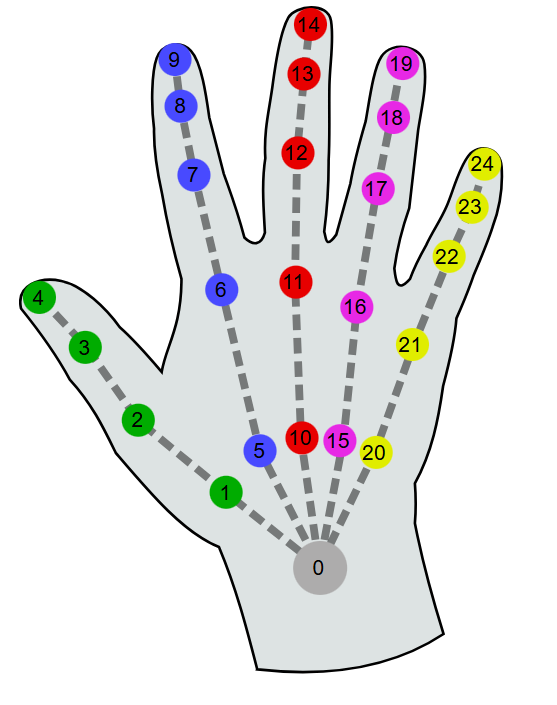
\includegraphics[width=0.4\textwidth]{img/webxr-mano.png} 
  \caption{Esquema manos}
  \label{fig:manos-esquema}
\end{figure}

Esto unicamente nos permite detectar las manos, pero no era suficiente para renderizarlas en la escena. Para ello era necesario crear una esfera por cada articulación. Utilizando el listado que posee todos los nombres de las articulaciones se crea una esfera por cada una y se procede a guardar cada entidad en un diccionario, a cada entidad se le asignaba un nombre con el nombre de la articulación y la mano a la que pertenece, definido en el \texttt{schema} del componente.

Ya que estabamos utilizando WebXR, para poder acceder a la información de las posiciones de cada articulación era necesario acceder a la sesion XR y acceder a sus inputs, en este caso las manos. Esto se realizaba en una función llamada \texttt{updateSkeleton}. Por cada input de la sesion el programa accede al diccionario creado anteriormente y por cada articulación, a traves de la sesion, se accede a su posición y tamaño y se actualiza la entidad correspondiente. También, en caso de que la articulación en cuestion sea la punta del deo índice o la muñeca se le añade un colisionador para 
poder interactuar con los elementos dentro de la escena. Esta actualización de la posición se realiza a cada frame, permitiendo un movimiento fluido y suave. 

Ahora que las manos se renderizan en la escena era necesario detectar los gestos. Para ello, en una función nueva llamada \texttt{detectGesture}, al igual que la anterior, esta función se ejecutaba a cada frame. Se vuelve a acceder a la sesión de WebXR para obtener las posiciones de algunas articulaciones clave, como la muñeca, las puntas de los dedos y la falanje intermedia del dedo índice.
Para el gesto \texttt{Pinch}, se utiliza la distancia entre la pinta del índice y del pulgar y si la distancia es lo suficiente pequeña o no se lanzan los eventos de \texttt{pinchstart} y \texttt{pinchend} respectivamente. Esta acción se ejecuta a traves de una función dentro de la función \texttt{detectGesture}, y lo mismo ocurre con los gestos de \texttt{Openhand} y \texttt{Fist}, pese a que luego no se usan estos gestos. El caso del gesto de \texttt{Point} es diferente al de los otros gestos, la forma en la que se detecta es igual, pero los otros gestos al lanzar sus eventos correspondientes, estos son escuchados por los componentes interactivos directamente, mientras que para este gesto,
dentro de este mismo componente se realizan varios pasos previos. Este gesto esta dividido en dos fases, cuando el usuario esta haciendo la acción de \texttt{pistol} y cuando no. Cuando no es cuando el usuario tiene el índice y el pulgar estirados, al realizar esta acción el programa crea un puntero en la punta del índice, este puntero es el que nos permite interactuar con los elementos a distancia. Cuando el usuario hace la acción de \texttt{pistol},cuando el pulgar se pega al dedo índice, haciendo la acción de disparar con los dedos, se emite el evento de \texttt{click} en el elemnto que intersecciona con el puntero. 

Para el puntero, era necesario que siguiera la dirección a la que puntamos con la mano, para ello en una tercera función llamada \texttt{updatePointer} se volvia a acceder a la sesión XR y se tomaban las posiciones de la punta y nudillo del dedo índice y usando el vector que se generaba a partir de esas posiciones se actualizaba la dirección a la que apunta el vector.

\subsection{Componentes interactivos}
\label{subsec:componentes-interactivos}
Para los componentes interactivos primero se creo el componente \texttt{grabable}, dicho componente era el encargado de escuchar los eventos de los colisionadores al igual que del gesto \texttt{Pinch}, al escuchar los eventos lo primero era diferenciar de que mano provenian, para ello en caso de colisión se comprueba el nombre de la articulación que colisionó y en el caso del gesto se comprueban los detalles del evento se introduce la mano definida en el \texttt{schema}. Dependiendo de la mano se actualiza una de las variables estado dentro de este componente. Independientemente de la mano, si se detecta una colisión,
se emite el evento de \texttt{hooverStart} y ya dependiendo de las variables estado que definen que mano esta colisionando o haciendo el gesto se emiten los eventos para realizar los gestos de \texttt{drag}, \texttt{slide} o \texttt{stretch}, estos eventos luego son escuchados por los componentes correspondientes a cada acción.

Para la acción de \texttt{click} es la única que no necesita pasar a traves del componente \texttt{grabable} ya que no es necesario tocar el elemento con este componente. 
Al recibir los eventos correspondientes a la acción, cambiando el color o devolviendolo a la normalidad dependiendo del evento. 
La acción de \texttt{hoover} al recibir sus eventos correspondietes hace que la entidad se vuelva mas transparente al interactuar con ella.
Para la acción de \texttt{slide}, al recibir el evento se accede a la información compartida a traves del evento, la posición del dedo índice, y dependeindo del eje seleccionado en el \texttt{schema} de este componente, se puede deslizar el elemento a traves de la escena en ese eje que selecciono el usuario mientras los otros ejes se mantienen constantes.

La acción de \texttt{drag} es la mas compleja de todas. Para que funcionase correctamente esta accion se divide en dos fases, el reparenting y la rotación. Para que el elemento de la escena pudiera ser cogido con la mano, al escuchar los eventos correspondientes se realiza un reparenting, haciendo que la entidad sea hija de la punta del dedo índice,su información se transmite en los detalles del evento, en vez de la escena, esto nos permite arrastrar la entidad por la escena. Pero por como se dibujan las articulaciones, unicamente se actualiza su posición y no la rotación era necesario un paso extra para la rotación.
Para ello primero se accede a la información de la mano, transmitida en los detalles del evento, y se toma la posicion de tres articulación, la punta y nudillo del índice y el nudillo del dedo meñique. Con esas tres posiciones se crea un eje relativo que posee la rotación de la mano, una vez con eso la entidad que estamos tomando copia dicho eje, haciendo que la entidad copie la rotación de la mano.
%%%%%%%%%%%%%%%%%%%%%%%%%%%%%%%%%%%%%%%%%%%%%%%%%%%%%%%%%%%%%%%%%%%%%%%%%%%%%%%%
%%%%%%%%%%%%%%%%%%%%%%%%%%%%%%%%%%%%%%%%%%%%%%%%%%%%%%%%%%%%%%%%%%%%%%%%%%%%%%%%
% PRUEBAS Y EXPERIMENTOS capitulo 5%
%%%%%%%%%%%%%%%%%%%%%%%%%%%%%%%%%%%%%%%%%%%%%%%%%%%%%%%%%%%%%%%%%%%%%%%%%%%%%%%%

\cleardoublepage
\chapter{Pruebas y experimentos}
\label{chap:pruebas-experimentos}
En este capítulo se describirán las distintas impresiones que han tenido familiares y amigos que han ayudado al probar la escena final. 

Primero se describirán las distintas instrucciones que se les dieron a cada uno nada más entrar a la escena y posteriormente se describirán las distintas impresiones y opiniones que han dado al respecto.
Para este apartado se pidió la colaboración de 4 familiares y amigos.

Nada más entrar a la escena, todos recibieron las mismas instrucciones. Lo primero era que se mirasen las manos para que las gafas pudieran detectarlas correctamente y el programa pudiera renderizarlas. Una vez las manos estaban ya renderizadas se les pidió que movieran sus manos y dedos y se les pidió que dieran su opinión al respecto. 
Las 4 personas dijeron cosas parecidas, que pese a que solo se renderizaban las articulaciones y no la mano en sí, la forma en la que se dibujaban y movían era bastante natural y fluida, pero algunos resaltaron que cuando las gafas no detectan bien algún dedo, ya sea porque algún objeto real o la propia mano está tapando un dedo, a veces dicho dedo realizaba movimientos extraños. 
Esto era de esperar, ya que dependemos del sistema de detección de manos de las gafas y si estas no detectan correctamente, el programa no puede funcionar correctamente. 

Luego de que se acostumbrasen a las manos virtuales, se les pidió que mirasen a su alrededor. Al cargar la escena el usuario aparece en el centro la escena y a su alrededor hay una serie de cubos formando un círculo. Cada cubo posee uno de los componentes interactivos que se han desarrollado y encima hay un panel con el nombre de este cubo, el cual refleja el componente que posee, y una descripción en inglés de lo que tienen que hacer para interactuar con él.
Únicamente aquellos que no eran fluidos con el inglés tuvieron ciertos problemas para entender las instrucciones de cada cubo, pero aquellos que lo entendían bien no tuvieron problemas. Uno por uno se acercaban a los cubos y mediante la acción correspondiente descrita en el panel, pudieron interactuar con todos y cada uno de los cubos. 

Una vez terminaron de experimentar con los distintos cubos de la escena, se les pidió que dieran su opinión al respecto. Todos estaban algo sorprendidos con la naturalidad con la que se movían las manos dentro de la escena al igual que les pareció bastante sencillo de interactuar con los distintos elementos de la escena, aunque recomendaron la implementación de nuevos gestos, ya que únicamente los gestos de \texttt{Pinch} y \texttt{Point} habían sido utilizados para los componentes.
%%%%%%%%%%%%%%%%%%%%%%%%%%%%%%%%%%%%%%%%%%%%%%%%%%%%%%%%%%%%%%%%%%%%%%%%%%%%%%%%
%%%%%%%%%%%%%%%%%%%%%%%%%%%%%%%%%%%%%%%%%%%%%%%%%%%%%%%%%%%%%%%%%%%%%%%%%%%%%%%%
% CONCLUSIONES capitulo 6%
%%%%%%%%%%%%%%%%%%%%%%%%%%%%%%%%%%%%%%%%%%%%%%%%%%%%%%%%%%%%%%%%%%%%%%%%%%%%%%%%

\cleardoublepage
\chapter{Conclusiones}
\label{chap:conclusiones}
En este último capítulo se presenta un resumen de las conclusiones obtenidas y las lecciones aprendidas a lo largo del desarrollo de este proyecto. También, se destacaran los conocimientos aplicados durante su elavoración y se evaluará el cumplimiento de los objetivos establecidos. Además, se ofreceran opciones y planteamientos de cara a futuras mejoras o implementaciones del sistema u otros posibles proyectos.

Respecto al cumplimiento del objetivo general, desarrollar un sistema de detección de manos y gestos para utilizar en escenas dentro del navegador, ha sido cumplido. Se ha creado un sistema de detección y renderización de manos capaz de interactuar con los distintos elementos dentro de la escena de forma mas natural y fluida en comparación a los elementos existentes previamente. La manos resultantes mantienen un tamaño y proporción bastante realistas respecto a las manos del usuario lo que le permite adaptarse mejor al entorno virtual.

Respecto a los objetivos específicos, tras realizar un estudio sobre las opciones actuales de detección de manos dentro de A-Frame, se llego a la conclusión de que la mejor opción era la de trabajar directamente con la información que nos proporciona WebXR. 
Utilizando esa información, se consigío cumplir los objetivos de detección y renderización de las manos dentro de la escena, al igual que la detección de gestos. 
Respecto a la implementación de acciones, ese objetivo se cumplio con creces. Al principio unicamente se planteaba implementar un par de acciones, pero al final del proyecto se logro implementar hasta 5 acciones, siendo estas las mismas que posee el componente de \texttt{Superhands}.
Finalmente se logro crear una escena donde el usuario sería capaz de experimentar el funcionameinto de los resultados de este proyecto, cumpliendo asi todos los objetivos planateados. 

\section{Aplicación de lo aprendido}
\label{sec:aplicacion}

En esta sección se detallan las distintas asignaturas de la carrera de Ingeniería en Sistemas Audiovisuales y Multimedia que han aportado los conocimientos necesarios para afrontar los distintos desafios que ha supuesto este proyecto. 

\begin{itemize}
  \item \textbf{Informática I y II:} Estas asignaturas fuero la base de todo. Me proporcionaron unos conocimientos fundamentales de la programa como la resolución de problemas mediante código o la programación oriendada a objetos.
  \item \textbf{Gráficos y Visualización en 3D:} Esta asignatura fue la que mas me ayudo de cara a este proyecto. Me proporcionó los conocimientos necesarios para dominar los principios básicos de la Visualización en 3D de un entorno virtual. También, me proporciono los conocimientos básicos de WebGL y de Three.js, herramientas que han sido esenciales durante todo el proyecto y sin las cuales no se habria podido completar. 
  \item \textbf{Construcción de servicios y aplicaciones audiovisuales en internet y Laboratorio de tecnoligías audiovisuales en la Web:} Estas dos asignaturas fueron mi primer contacto con la programación web. Me dieron los conocimientos esenciales de HTML, CSS y JavaScript necesarios para la creación de páginas web dinámicas e interactivas, permitiendo asi la creación de las distintas escenas demo y de la lógica detras de todos los componentes que permiten que funcione el proyecto.
\end{itemize}

\section{Lecciones aprendidas}
\label{sec:lecciones_aprendidas}

A lo largo del desarrollo de este Trabajo de Fin de Grado, me he enfrentado a diversos obstáculos los cuales al superarlos, me han aportado nuevos conocimientos sobre las tecnologías utilizadas en este proyecto, además, también los conocimientos que tenía previamente que han sido aplicados a este proyecto han mejorado y me han dado un mayor entendimiento de las tecnologías utilizadas.

Gracias a este proyecto, aprendí a manejar tecnologías como A-Frame, WebGL y WebXR. Esta era mi primera experiencia con el mundo de la realidad virtual, sobre todo como desarrollador, pero gracias a las tecnologías mencionadas, aprendí a crear escenas inmersivas e interactivas. También aprendí a manejar la lógica necesaria para detectar cambios que ocurrían a cada frame dentro de la escena, como el cambio de las posiciones de las manos o los gestos y a responder a dichos cambios de la forma deseada mediante eventos. 
Aparte, también obtuve conocimientos sobre el manejo del DOM y la manipulación de elementos HTML con el fin de crear experiencias interactivas. La integración de estos elementos me ayudo a comprender como los usuarios podían interactuar de manera más natural con los elementos virtuales dentro de la escena.

Además, mi manejo de GitHub ha mejorado gracias a este proyecto, he aprendido a mantener mi código más ordenado y limpio, aparte del uso de GitHub pages, que me ha permitido crear páginas web donde visualizar las distintas demos que se fueron creando. También aprendí a utilizar LaTeX para la creación de la documentación de este proyecto. Esta herramienta me ha ayudado a producir un documento técnico de alta calidad, permitiendo estructurar de forma clara y precisa los distintos aspectos del proyecto mientras mantiene una presentación ordenada y profesional. 

\section{Trabajos futuros}
\label{sec:trabajos_futuros}
Aunque este proyecto ha conseguido sus objetivos, aún tiene mucho espacio para mejora. A continuación se presentan algunas de las posibles mejoras que se le podrían realizan al proyecto para mejorarlo y como esta tecnología puede ser aplicada en distintas aplicaciones o escenas virtuales:

\begin{itemize}
  \item \textbf{Desarrollo de nuevas poses:} En este proyecto en el resultado final únicamente se han implementado un par de gestos, pero dada la forma en la que se obtiene la información de WebXR, no resultaría muy complejo implementar nuevos para añadir mayor profundidad a la experiencia de inmersión.
  \item \textbf{Desarrollo de nuevas acciones:} Del mismo modo que con los gestos, es posible crear nuevos componentes para realizar distintos tipos de acciones que permitan aumentar las distintas formas que tiene el usuario para interactuar con la escena.
  \item \textbf{Implementar soporte para realidad aumentada:} Actualmente el sistema desarrollado en este proyecto únicamente funciona en entornos VR, pero se puede llegar a configurar para que también funcione en entornos AR.
  \item \textbf{Mejora de la detección de poses:} Aunque el sistema detecta generalmente la pose que se está realizando, es posible mejorar la lógica detrás de esto para que sea más preciso aún.
  \item \textbf{Implementar compatibilidad con controladores:} Dado que existen sistemas que realizan cosas similares que las manos desarrolladas en este proyecto utilizando los controladores, es posible llegar a configurar el código para que dentro de la misma escena sea posible utilizar tanto las manos como los controladores funcionen de forma conjunta. Una opción sería combinar el código con el componente de \texttt{Superhands}.
  \item \textbf{Implementaciones:} La posibilidad de poder visualizar tus manos reales dentro del entorno virtual y de poder interactuar con estas con los distintos elementos de la escena da paso a posibilidades casi infinitas. Algunos ejemplos de posibles implementaciones sería la del uso en videojuegos, la creación de aplicaciones de diseño o incluso simuladores de entrenamiento para distintas profesiones.
\end{itemize}
%%%%%%%%%%%%%%%%%%%%%%%%%%%%%%%%%%%%%%%%%%%%%%%%%%%%%%%%%%%%%%%%%%%%%%%%%%%%%%%%
%%%%%%%%%%%%%%%%%%%%%%%%%%%%%%%%%%%%%%%%%%%%%%%%%%%%%%%%%%%%%%%%%%%%%%%%%%%%%%%%
% BIBLIOGRAFIA %
%%%%%%%%%%%%%%%%%%%%%%%%%%%%%%%%%%%%%%%%%%%%%%%%%%%%%%%%%%%%%%%%%%%%%%%%%%%%%%%%

\cleardoublepage

% Las siguientes dos instrucciones es todo lo que necesitas
% para incluir las citas en la memoria
\bibliographystyle{abbrv}
\bibliography{memoria} 

\end{document}
